%----------------------------------------------------------------------------------------
%    PACKAGES AND THEMES
%----------------------------------------------------------------------------------------

\documentclass[aspectratio=169,xcolor=dvipsnames]{beamer}
\usetheme{SimpleDarkBlue}

\usepackage{hyperref}
\usepackage{graphicx} % Allows including images
\usepackage{booktabs} % Allows the use of \toprule, \midrule and \bottomrule in tables
\usepackage{subcaption}
\usepackage{tikz}
\usepackage{natbib}

\usepackage{bbm}
\usepackage[normalem]{ulem}

\usetikzlibrary{arrows.meta, positioning, shapes, calc}

%----------------------------------------------------------------------------------------
%    TITLE PAGE
%----------------------------------------------------------------------------------------

\title{On Regularization of Maximum Mean Discrepancy \\ Gradient Flow}

\author{
Zonghao Chen \and
Aratrika Mustafi \and
Pierre Glaser \and Anna Korba \\
\and Arthur Gretton \and Bharath K. Sriperumbudur
}

\date[]{}
% Date, can be changed to a custom date

\usepackage{amsthm}
\newtheorem{thm}{Theorem}
\newtheorem{cor}[theorem]{Corollary}
\newtheorem{lem}[theorem]{Lemma}
\newtheorem{prop}[theorem]{Proposition}
\newtheorem{rem}[theorem]{Remark}
\newtheorem{defi}{Definition}
\newtheorem{ass}{Assumption}



\definecolor{definitionTitle}{RGB}{34, 102, 102}  % A deep teal color
\definecolor{definitionBody}{RGB}{10, 10, 10}     % Near-black for text
\definecolor{answerBody}{RGB}{225, 244, 244}

\setbeamercolor{block title alerted}{bg=brown, fg=white}
\setbeamercolor{block body alerted}{fg=definitionBody}
\setbeamercolor{answer box}{bg=answerBody, fg=black}

% Now redefine the 'defi' environment to use the 'alerted block' style:
\setbeamertemplate{theorems}[numbered]
\let\olddefi\defi
\renewenvironment{defi}[1][]{%
  \begin{alertblock}{Definition\ifx\\#1\\\else~(#1)\fi}%
}{%
  \end{alertblock}%
}

\newenvironment{answerblock}{%
  \begin{beamercolorbox}[wd=\linewidth, sep=0.15em, rounded=true, shadow=true]{answer box}%
}{%
  \end{beamercolorbox}%
}

\definecolor{graytext}{gray}{0.5} % Customize the grey level if needed
\definecolor{darkgreen}{RGB}{0, 100, 0}
% Save the original versions
\let\oldcitep\citep

% Use compact, unobtrusive citations throughout the slides.
\renewcommand{\citep}[1]{{\scriptsize\textcolor{graytext}{\oldcitep{#1}}}}
\renewcommand{\cite}[1]{{\scriptsize\textcolor{graytext}{\oldcitep{#1}}}}
\newcommand{\red}[1]{\textcolor{red}{#1}}
\newcommand{\green}[1]{\textcolor{darkgreen}{#1}}
\newcommand{\orange}[1]{\textcolor{orange}{#1}}
\newcommand{\blue}[1]{\textcolor{blue}{#1}}

\newcommand{\authorportrait}[2]{%
    \begin{minipage}[t]{0.155\textwidth}
        \centering
        \begin{tikzpicture}
            \clip (0,0) circle (0.72cm);
            \node at (0,0) {\includegraphics[width=1.44cm,height=1.44cm]{#1}};
        \end{tikzpicture}\\[-1pt]
        {\scriptsize #2}
    \end{minipage}%
}

\newenvironment{talign*}
 {\let\displaystyle\textstyle\csname align*\endcsname}
 {\endalign}
\newenvironment{talign}
 {\let\displaystyle\textstyle\csname align\endcsname}
 {\endalign}

%----------------------------------------------------------------------------------------
%    PRESENTATION SLIDES
%----------------------------------------------------------------------------------------

\begin{document}

\newcommand{\E}{\mathbb{E}}
\newcommand{\R}{\mathbb{R}}
\newcommand{\Qb}{\mathbb{Q}}
\newcommand{\Pb}{\mathbb{P}}
\newcommand{\calH}{\mathcal{H}}
\newcommand{\calN}{\mathcal{N}}
\newcommand{\calM}{\mathcal{M}}
\newcommand{\calE}{\mathcal{E}}
\newcommand{\calT}{\mathcal{T}}
\newcommand{\calL}{\mathcal{L}}
\newcommand{\calF}{\mathcal{F}}
\newcommand{\calG}{\mathcal{G}}
\newcommand{\calZ}{\mathcal{Z}}
\newcommand{\calO}{\mathcal{O}}
\newcommand{\calX}{\mathcal{X}}
\newcommand{\calP}{\mathcal{P}}
\newcommand{\dd}{\mathrm{d}}
\newcommand{\bx}{\mathbf{x}}
\newcommand{\bo}{\mathbf{o}}
\newcommand{\by}{\mathbf{y}}
\newcommand{\bz}{\mathbf{z}}
\newcommand{\bH}{\mathbf{H}}
\newcommand{\bw}{\mathbf{w}}
\newcommand{\bJ}{\mathbf{J}}
\newcommand{\bnabla}{\boldsymbol{\nabla}}
\newcommand{\scrG}{\mathscr{G}}
\newcommand{\scrF}{\mathscr{F}}
\newcommand{\scrX}{\mathscr{X}}
\newcommand{\scrx}{\mathscr{X}}
\newcommand{\scrY}{\mathscr{Y}}
\newcommand{\scry}{\mathscr{Y}}
\newcommand{\scrZ}{\mathscr{Z}}
\newcommand{\scrz}{\mathscr{Z}}
\newcommand{\scrU}{\mathscr{U}}
\newcommand{\scrR}{\mathscr{R}}
\newcommand{\scrQ}{\mathscr{Q}}
\newcommand{\scrL}{\mathscr{L}}

\newcommand{\Id}{\mathrm{Id}}
\newcommand{\N}{\mathbb{N}}
\newcommand{\kl}{\mathrm{KL}}
\newcommand{\tv}{\mathrm{TV}}
\newcommand{\LSI}{\mathrm{LSI}}
\newcommand{\mmd}{\mathrm{MMD}}
\newcommand{\ksd}{\mathrm{KSD}}
\newcommand{\dmmd}{\mathrm{DrMMD}}

\newcommand{\one}{\mathbbm{1}}

\begin{frame}[plain]
    \centering
    \vfill
    {\usebeamerfont{title}\color{DarkBlue}\inserttitle\par}
    \vfill
\end{frame}


%------------------------------------------------
\section{Background}
%------------------------------------------------
\begin{frame}{Background}
\large
\begin{exampleblock}{}
\centering
    \textbf{Problem}: How to learn a target probability distribution $\pi$ on $\R^d$.
\end{exampleblock}
\begin{itemize}
    \item Sampling (e.g: $\pi\propto\exp(-V)$ is the posterior distribution in Bayesian inference). 
    \item Generative models (e.g: $\pi$ is the distribution of an image dataset). 
\end{itemize}
\begin{columns}[T,totalwidth=0.86\textwidth]
    \column{0.29\textwidth}
    \vspace{0pt}
    \raggedleft
    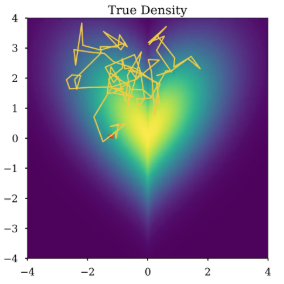
\includegraphics[height=0.29\textheight,trim=0 25bp 15bp 25bp,clip]{figures/sampling.png}

    \column{0.55\textwidth}
    \vspace{0pt}
    \raggedright
    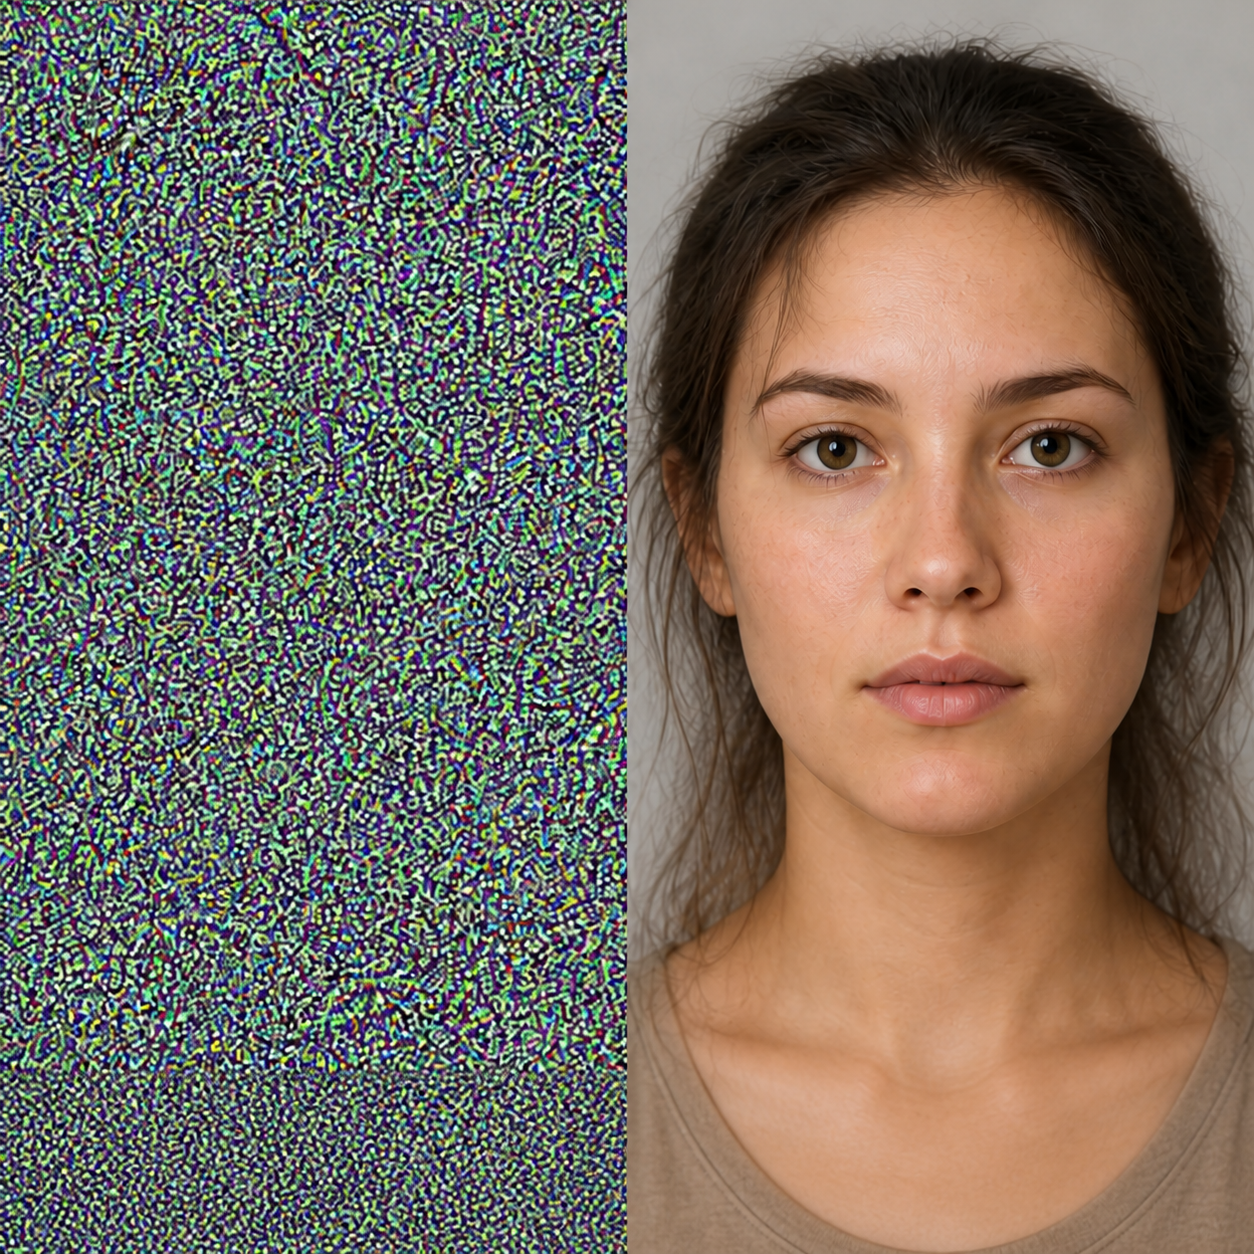
\includegraphics[height=0.29\textheight,trim=0 313.5bp 627bp 313.5bp,clip]{figures/generative_noise_to_face.png}
    \hspace{0.10cm}
    \raisebox{0.115\textheight}{\LARGE$\rightarrow$}
    \hspace{0.10cm}
    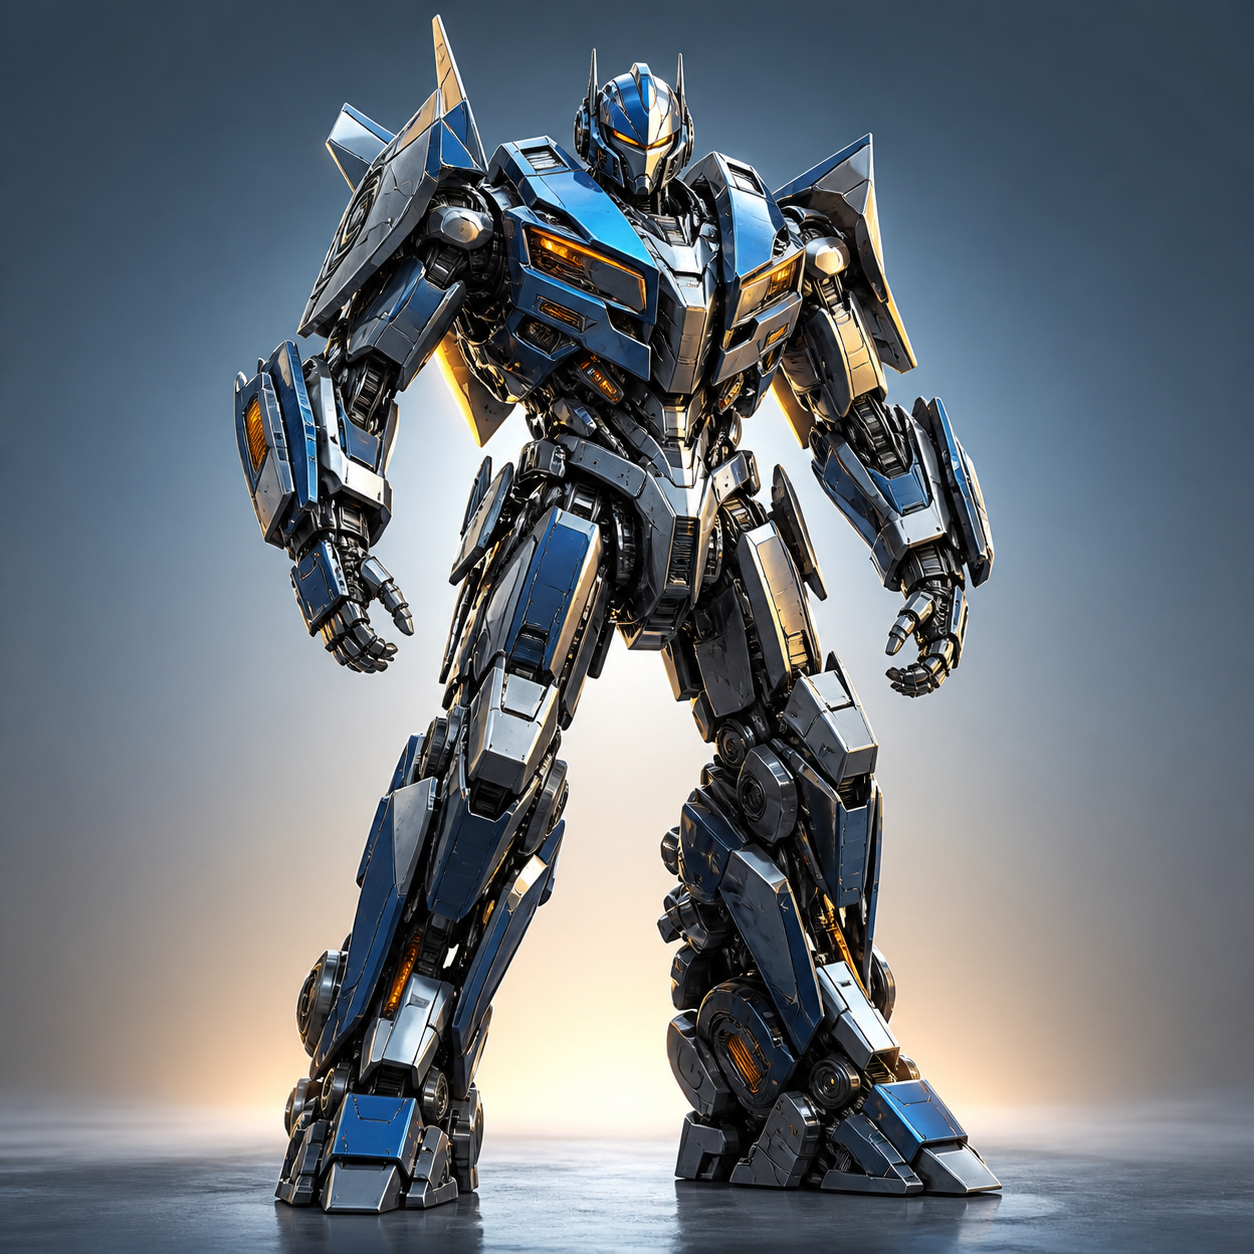
\includegraphics[height=0.29\textheight]{figures/generative_transforming_robot.png}
\end{columns}
\end{frame}


\begin{frame}{Background: Optimization in the space of probability measures}
    \begin{exampleblock}{}
    \centering
        \textbf{Problem}: How to learn a target probability distribution $\Qb$ on $\R^d$.
    \end{exampleblock}
    \begin{itemize}
        \item This problem can be written as an \blue{optimization} problem on $\calP_2(\R^d)$.
        \begin{talign*}
            \arg\min_{\Pb \in \calP_2(\R^d)} D(\Pb \mid \Qb) .
        \end{talign*}
        \item Here $D$ is a similarity metric or distance, e.g. Kullback–Leibler divergence.
        \begin{itemize}
            \item $D(\Pb | \Qb) = 0$ if and only if $\Pb=\Qb$.
        \end{itemize}
        \item \red{$\calP_2(\R^d)$ denotes the space of probability measures with a finite second moment}.
        \begin{itemize}
            \item We primarily consider $\calP_2(\R^d)$ rather than $\calP(\R^d)$ for the nice geometrical properties.
        \end{itemize}
        \item How to find the minimum? Gradient descent!
    \end{itemize}
\end{frame}


\begin{frame}{Background: Euclidean gradient flow}
    \begin{itemize}
        \item Euclidean gradient flow of an objective $F:\R^d \to \R$
        \begin{talign*}
            \partial_t x_t = -v(x_t), \quad v = \nabla F .
        \end{talign*}
        \item $\nabla F$ denotes the gradient of $F$.
        \item This is the continuous-time analogue of gradient descent: \begin{talign*}
            x_{n+1} = x_n - \gamma v(x_n),
        \end{talign*}
        where $\gamma > 0$ is the step size.
        \item When $F$ is both \green{strongly convex and smooth}, Euclidean gradient \orange{descent} converges exponentially fast~\citep{boyd2004convex}.
    \end{itemize}
\end{frame}



\begin{frame}{Background: Wasserstein gradient flow}
    \begin{exampleblock}{}
    \centering
        \textbf{Challenge}: How to find $\arg\min_{\Pb \in \calP_2(\R^d)} D(\Pb \mid \Qb)$?
    \end{exampleblock}
    \begin{itemize}
        \item Gradient descent! Wait... How do we define gradients in $\calP_2(\R^d)$?
        \item Endow $\calP_2(\R^d)$ with the Wasserstein-2 distance $W_2$.
        \begin{talign*}
            \red{W_2^2(\nu, \Pb)} = \smallint \| T(x) - x\|^2 \dd \nu(x) = \| T - \Id\|_{L_2(\nu)}^2 .
        \end{talign*}
        \vspace{-10pt}
        \begin{itemize}
            \item $W_2^2(\nu, \Pb)$ means the \orange{minimal energy} takes to transport mass from $\nu$ to $\Pb$.
            \item $T:\R^d\to\R^d$ is the \red{optimal transport map} from $\nu$ to $\Pb$.
        \end{itemize}
        \item $(\calP_2, W_2)$ can be 'treated` as a Riemann manifold under Otto's calculus~\citep{otto2001geometry}.
        \item The \green{tangent space} $\calT_\Pb\calP_2(\R^d)$ at $\Pb\in\calP_2(\R^d)$ is a dense subset of $L_2(\Pb)$.
    \end{itemize}
    \begin{figure}
        \centering
        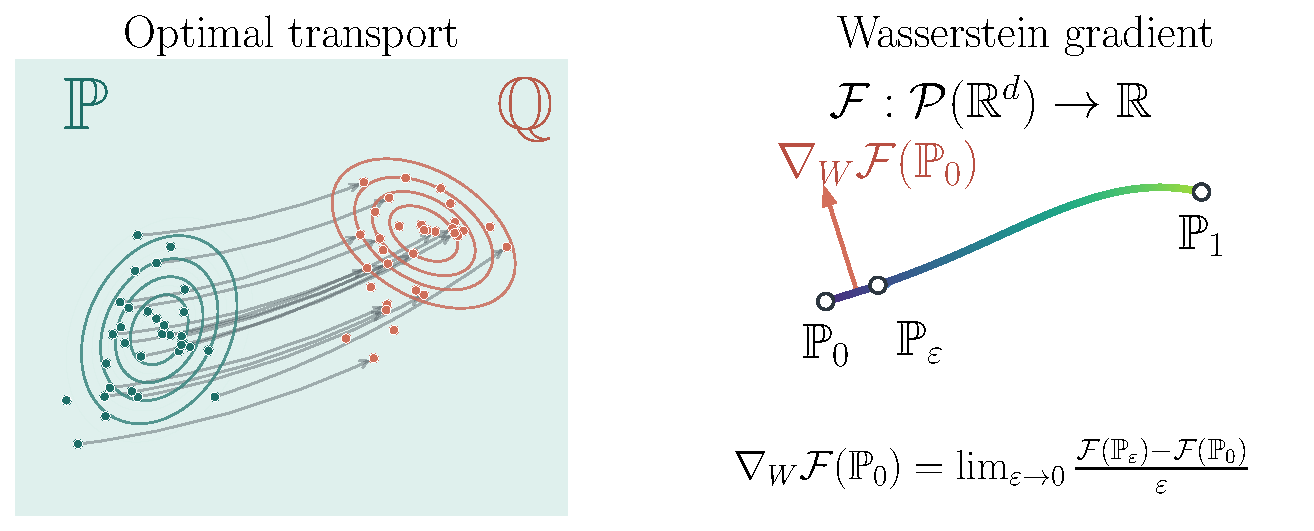
\includegraphics[
            height=0.24\textheight,
            trim=0 0 315bp 0,
            clip
        ]{figures/ot_wasserstein_gradient_illustration.pdf}
        \hspace{0.04\linewidth}
        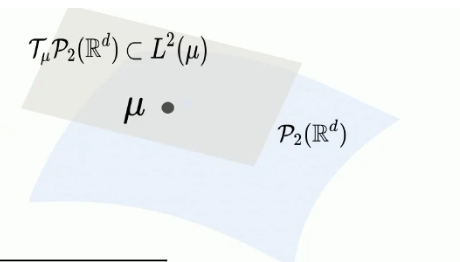
\includegraphics[height=0.24\textheight]{figures/tangent.png}
    \end{figure}
\end{frame}

\begin{frame}{Background: Wasserstein gradient flow}
    \vspace{-0.18cm}
    \begin{figure}
        \centering
        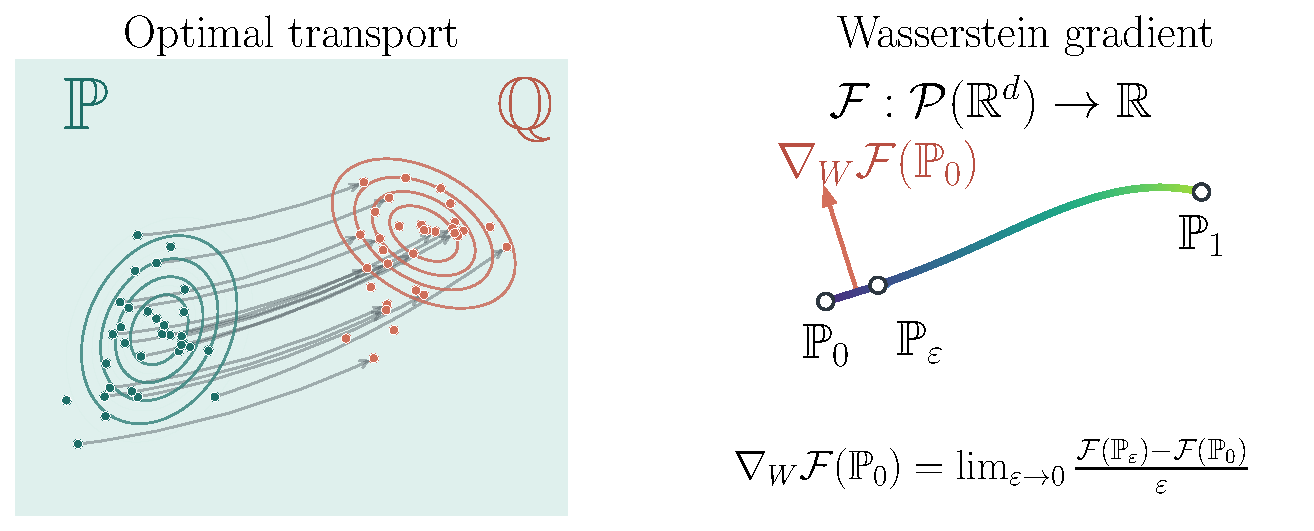
\includegraphics[
            width=0.27\linewidth,
            trim=315bp 60bp 0 0,
            clip
        ]{figures/ot_wasserstein_gradient_illustration.pdf}
    \end{figure}
\begin{defi}[Wasserstein gradient]
Let $\calF: \calP_2(\R^d) \rightarrow \R$.
The \red{Wasserstein gradient of $\calF$} evaluated at $\Pb \in \calP_2(\R^d)$ is the unique function \blue{$\nabla_{W_2} \calF(\Pb): \R^d \rightarrow \R^d$}, s.t. for any $T\in \calT_\Pb\calP_2(\R^d)$,
\begin{align*}
\lim _{\epsilon \rightarrow 0} \frac{1}{\epsilon}\left[\calF\left( (\Id+\epsilon T)_\# \Pb \right) - \calF(\Pb)\right] = \left\langle \nabla_{W_2} \calF, T \right\rangle_{L_2(\Pb)} .
\end{align*}
\end{defi}
\begin{itemize}
    \item The gradient is defined along a `curve' $(\Id+\epsilon T)_\# \Pb$ in $\calP_2(\R^d)$.
\end{itemize}
\end{frame}

\begin{frame}{Background: Wasserstein gradient  flow}
\begin{defi}[Wasserstein gradient  flow]
\red{Wasserstein gradient flow} of $\calF:\calP_2(\R^d)\to\R$ is a sequence of distributions $(\Pb_t)_{t\geq 0}$ that evolves according to the \red{continuity equation} $\partial_t \Pb_t+\nabla \cdot \left(\Pb_t v_t\right)=0$,
where the vector field $v_t = -\nabla_{W_2}\calF(\Pb_t)$.
Or equivalently, $\dot{x}_t = v_t(x_t)$ with $\Pb_t = \mathrm{Law}(x_t)$.
\end{defi}
\begin{columns}[T]
    \column{0.48\textwidth}
    \textbf{Euclidean Gradient Flow}
    \begin{itemize}
        \item State space: $\R^d$
        \item Objective $F: \R^d \to \R$.
        \item Update scheme: $\dot{x}_t = v_t(x_t)$, with $v_t = -\nabla F$.
    \end{itemize}

    \column{0.48\textwidth}
    \textbf{Wasserstein Gradient Flow}
    \begin{itemize}
        \item State space: $\calP_2(\R^d)$
        \item Objective $\calF: \calP_2(\R^d) \to \R$:
        \item Update scheme $\dot{x}_t = v_t(x_t)$, with $v_t = -\nabla_{W_2} \calF(\Pb_t)$.
    \end{itemize}
\end{columns}
\end{frame}

\section{Examples of WGF}
\begin{frame}{Example 1: Langevin diffusion~\citep{jordan1998variational}}
    \begin{itemize}
        \item Given the target distribution $\Qb\propto \exp(-V)$ with $V: \R^d\to\R$.
        \item The functional \textcolor{blue}{$\calF_\kl = \kl(\cdot, \Qb)$} and its Wasserstein gradient
        \begin{talign*}
            \red{[\nabla_{W_2} \calF_\kl(\Pb)](\cdot)} = \nabla V(\cdot) + \nabla \log \Pb_t(\cdot) .
        \end{talign*}
        \item The Wasserstein gradient flow of $\calF_\kl$
        \begin{talign*}
            \partial_t \Pb_t=\nabla \cdot \left(\Pb_t \left( \nabla V + \nabla \log \Pb_t\right) \right).
        \end{talign*}
        \item It is equivalent to the Fokker–Planck equation of the \green{Langevin diffusion}~\citep{sarkka2019applied}:
        \begin{talign*}
            \dd x_t = -\nabla V(x_t) \, \dd t + \sqrt{2} \, \dd W_t, \quad \Pb_t = \mathrm{Law}(x_t).
        \end{talign*}
        \item A standard time-discretization (Euler--Maruyama scheme) is:
        \[
        x_{n+1} = x_n - \gamma \nabla V(x_n) + \sqrt{2\gamma} \, \xi_n, \quad \xi_n \sim \mathcal{N}(0, \Id_d).
        \]
    \end{itemize}
\end{frame}

\begin{frame}{Background: Maximum Mean Discrepancy (MMD)~\citep{gretton2012kernel}}
    \begin{columns}[c,onlytextwidth]
        \column{0.72\textwidth}
        \begin{itemize}
            \item $\calH$ is a reproducing kernel Hilbert space (RKHS) with kernel $k$.
            \begin{align*}
                \mmd(\Pb, \Qb)
                := \sup_{f \in \calH}
                |\E_{\Pb}[f(X)] - \E_{\Qb}[f(X)]|.
            \end{align*}
            \item The RKHS contains functions that are linear combinations of the feature maps $\phi:\calX\to\calH$, $f=\sum_{i=1}^n \alpha_i \phi(x_i)$.

        \end{itemize}

        \column{0.27\textwidth}
        \centering
        \begin{tikzpicture}[scale=0.72, every node/.style={font=\scriptsize}]
            \begin{scope}
                \draw[->, thick] (-1.55,0) -- (1.75,0) node[right] {$x$};
                \node[above] at (0.1,0.38) {input space};

                \foreach \x in {-0.9,-0.65,-0.35,-0.1} {
                    \fill[blue!80!black] (\x,0) circle (2pt);
                }
                \foreach \x in {0.45,0.7,1.0,1.25} {
                    \fill[orange!90!black] (\x,0) circle (2pt);
                }
                \node[blue!80!black] at (-0.55,-0.35) {$\Pb$};
                \node[orange!90!black] at (0.95,-0.35) {$\Qb$};
            \end{scope}
            \vspace{0.2cm}
            \begin{scope}[shift={(0,-2.55)}]
                \draw[->, thick] (-1.55,0) -- (1.75,0) node[right] {$\phi_1$};
                \draw[->, thick] (-1.35,-1.1) -- (-1.35,1.25) node[above] {$\phi_2$};
                \node[above] at (0.15,1.25) {feature space};

                \foreach \p in {(-1.0,0.55),(-0.72,0.82),(-0.35,0.48),(-0.05,0.9)} {
                    \fill[blue!80!black] \p circle (2pt);
                }
                \foreach \p in {(0.25,-0.45),(0.58,-0.2),(0.95,-0.52),(1.25,-0.05)} {
                    \fill[orange!90!black] \p circle (2pt);
                }
            \end{scope}
        \end{tikzpicture}
    \end{columns}
    \begin{thm}{MMD admits a closed-form expression}
        \small
        \begin{align*}
            \mmd^2(\Pb, \Qb)
            = \E_{X,X'\sim\Pb}[k(X,X')]
            + \E_{Y,Y'\sim\Qb}[k(Y,Y')] - 2\E_{X\sim\Pb,\,Y\sim\Qb}[k(X,Y)] .
        \end{align*}
    \end{thm}
    \begin{itemize}
        \item MMD is a probability divergence ($\mmd(\Pb, \Qb)=0 \iff \Pb=\Qb$) if $k$ is characteristic (Gaussian)~\citep{sriperumbudur2011universality}.
    \end{itemize}
\end{frame}

\begin{frame}{Example 2: MMD gradient flow~\citep{arbel2019maximum}}
\begin{itemize}
    \item The functional \textcolor{blue}{$\calF_\mmd = \frac{1}{2}\mmd^2(\cdot, \Qb)$}
    \item Its Wasserstein gradient
    \begin{align*}
        \red{[\nabla_{W_2} \calF_\mmd(\Pb)](\cdot)} &= \nabla \Big( \smallint k(x, \cdot) \; \dd \Pb(x) - \smallint k(x, \cdot) \; \dd \Qb(x) \Big) .
    \end{align*}
    \item The Wasserstein gradient flow of $\calF_\mmd$,
    \begin{talign*}
        \partial_t \Pb_t=\nabla \cdot \left(\Pb_t \nabla_{W_2} \calF_\mmd(\Pb_t) \right), \quad  \dd x_t = -[\nabla_{W_2} \calF_\mmd(\Pb_t)](x_t) \, \dd t .
    \end{talign*}
    \item A standard time-discretization (Euler--Maruyama scheme) is:
    \[
    x_{n+1} = x_n - \gamma \nabla_{W_2} \calF_\mmd(\Pb_n)(x_n) , \quad \text{Law}(x_n)=\Pb_n.
    \]
    \item The same holds for $\calF_\ksd = \frac{1}{2}\mmd^2(\cdot, \Qb)$ with a Stein kernel $k_\Qb$~\citep{korba2021kernel}.
\end{itemize}
\end{frame}




\begin{frame}{Convergence}
    \begin{columns}[T]
    \column{0.48\textwidth}
    \textbf{Wasserstein gradient flow of $\calF_\kl$}
    \begin{itemize}
        \item $\Qb\propto\exp(-V)$
        \item Sampling
        \item Convergence in discrete time
        \begin{align*}
            \kl(\Pb_n,\Qb)
            &\leq \exp(-\beta^{-1}\gamma n)\kl(\Pb_0,\Qb) \\
            &\quad + \gamma n L^2\beta.
        \end{align*}
        \item $\beta^{-1}$ is the LSI constant of $\Qb$, and $L$ is the Lipschitz constant of $\nabla V$.
        \item \blue{$\lim_{n\to\infty} \kl(\Pb_n, \Qb) = 0$!}.
    \end{itemize}

    \column{0.48\textwidth}
    \textbf{Wasserstein gradient flow of $\calF_\mmd$}
    \begin{itemize}
        \item $\{y_i\}_{i=1}^M$ i.i.d samples from $\Qb$
        \item Generative modelling
        \item \textcolor{blue}{Non-}convergence in discrete time
        \begin{talign*}
            \mmd^2(\Pb_n, \Qb) \leq \frac{W_2^2(\Pb_0,\Qb)}{\gamma n} + \bar{K}.
        \end{talign*}
        \item $\bar{K}$ is a positive barrier term that does not vanish.
        \item \blue{$\lim_{n\to\infty} \mmd(\Pb_n, \Qb) \neq 0$!}
    \end{itemize}
\end{columns}
\end{frame}

\section{DrMMD}

\begin{frame}{Non-convexity of MMD prevents global convergence}
    \begin{figure}
        \centering
        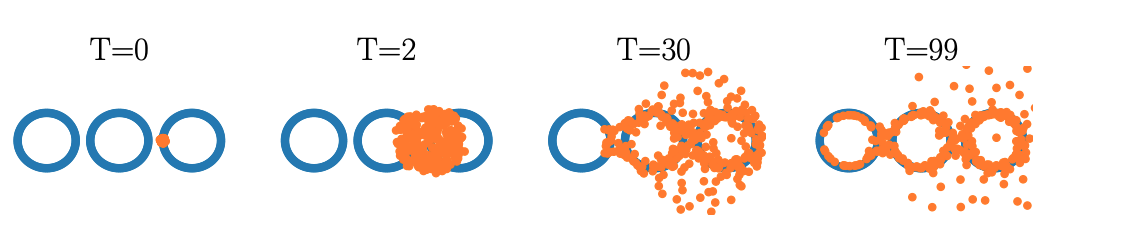
\includegraphics[width=0.6\linewidth]{figures/nonceonvxity_mmd.png}
    \end{figure}
    \vspace{-15pt}
    \begin{figure}
        \centering
        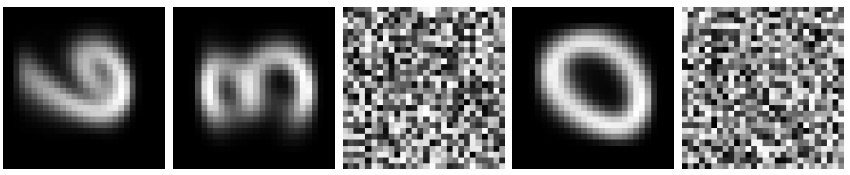
\includegraphics[width=0.6\linewidth]{figures/blurry_images_mmd.png}
        \caption{\citep{belhadji2025weighted}}
    \end{figure}
    \vspace{-10pt}
    \begin{itemize}
        \item Convergence of MMD flow has been proved under noise injection and stringent conditions on the noise scale~\citep{arbel2019maximum,chen2025stationary}.
        \item Disclaimer: There exists many papers where MMD flow \green{empirically} generate high-quality images with adversarial training of kernels~\citep{galashov2024deep}, or with non-smooth kernels plus deep network distillation~\citep{hertrich2023generative,altekruger2023neural}.
    \end{itemize}
\end{frame}

\begin{frame}{Non-convexity of MMD prevents global convergence}
    \begin{exampleblock}{}
        \centering
        \textbf{Question}: How can we overcome the non-convexity of $\calF_\mmd$?
    \end{exampleblock}
    \begin{itemize}
        \item In this talk, I will present three complementary routes.
    \end{itemize}
    \vspace{0.18cm}
    \begin{center}
        {\Large\blue{\textbf{1. De-regularized MMD gradient flow}}}\\[0.08cm]
        {\href{https://arxiv.org/abs/2409.14980}{\texttt{arXiv:2409.14980}}}\\[0.38cm]
        {\Large\green{\textbf{2. Sobolev-regularized MMD gradient flow}}}\\[0.08cm]
        {\href{https://arxiv.org/abs/2605.11884}{\texttt{arXiv:2605.11884}}}\\[0.38cm]
        {\Large\orange{\textbf{3. Applications: 1) Statistical inference; 2) Generative model}}}\\[0.08cm]
        {\scriptsize}{\texttt{arXiv:2607.03871}, \emph{Work in progress}}
    \end{center}
\end{frame}

\subsection{DrMMD flow and SrMMD flow}
\begin{frame}[plain]
    \centering
    \vfill
    {\usebeamerfont{title}\color{DarkBlue}DrMMD flow and SrMMD flow\par}
    \vspace{0.75cm}

    \authorportrait{figures/authors/zonghao.jpg}{Zonghao\\Chen}\hfill
    \authorportrait{figures/authors/aratrika.jpg}{Aratrika\\Mustafi}\hfill
    \authorportrait{figures/authors/pierre.jpg}{Pierre\\Glaser}\hfill
    \authorportrait{figures/authors/anna.jpg}{Anna\\Korba}\hfill
    \authorportrait{figures/authors/arthur.png}{Arthur\\Gretton}\hfill
    \authorportrait{figures/authors/bharath.jpg}{Bharath K.\\Sriperumbudur}
    \vfill
\end{frame}

\begin{frame}{Kernel assumptions}
\begin{ass}[Growth I]
There exists a constant $M>0$ such that, for every $x\in\R^d$,
\begin{align*}
    \lvert k(x,x)\rvert
    &\leq M\left(1+\lvert x\rvert^4\right), \\
    \left\lvert \partial_{1,i}\partial_{2,i}k(x,x)\right\rvert
    &\leq M\left(1+\lvert x\rvert^2\right), \qquad i\in[d].
\end{align*}
\end{ass}

\begin{ass}[Local Boundedness]
For $R>0$, let $\mathcal K=B(0,R)\subset\R^d$. There exists a $B_R>0$ such that, for every $i,j\in[d]$,
\begin{align*}
    \sup_{x\in\mathcal K}
    \left| \partial_{1,i}\partial_{1,j} \partial_{2,i} \partial_{2,j} k(x, x) \right| \leq B_R.
\end{align*}
\end{ass}
\begin{itemize}
    \item Gaussian, Mat\'{e}rn, and inverse multiquadratic kernels.
    \item Polynomial kernels.
    \item Stein kernels with score functions of at most linear growth.
\end{itemize}
\end{frame}

\begin{frame}{DrMMD: motivation}

\begingroup
\small
\setlength{\abovedisplayskip}{3pt}
\setlength{\belowdisplayskip}{3pt}
$T_\Qb: L_2(\Qb)\to L_2(\Qb)$ is the kernel \red{integral operator} defined as
\begin{align*}
    T_\Qb f(\cdot)=\int k(x,\cdot)f(x)\;\dd\Qb(x) .
\end{align*}
\endgroup
\vspace{-0.12cm}

\begin{prop}[MMD and $\chi^2$-divergence]
Suppose $\Pb$ is absolutely continuous with respect to $\Qb$, i.e., $\Pb \ll \Qb$. Then
\vspace{-10pt}
\begin{talign*}
    \mmd^2(\Pb, \Qb)=\left\|T_\Qb^{\frac{1}{2}} \left(\frac{\dd \Pb}{\dd \Qb}-1\right)\right\|_{L_2(\Qb)}^2 \text { and } \chi^2(\Pb, \Qb)=\left\|\frac{\dd \Pb}{\dd \Qb}-1 \right\|_{L_2(\Qb)}^2 .
\end{talign*}
\end{prop}
\begin{itemize}
    \item Similar to $\calF_\kl$, $\calF_{\chi^2}(\cdot)=\chi^2(\cdot, \Qb)$ flow enjoys convergence for Gaussian-like $\Qb$~\citep{ohta2011displacement}.
    \item An \green{interpolation} between $\mmd^2$ and $\chi^2$?
\end{itemize}
\end{frame}


\begin{frame}{DrMMD: An interpolation of MMD and $\chi^2$}
\begin{defi}[De-regularized Maximum Mean Discrepancy (DrMMD)]
Suppose $\Pb\ll\Qb$ where $\Pb, \Qb \in \calP_2(\R^d)$. Then the (de)-regularized maximum mean discrepancy (DrMMD) between $\Pb, \Qb$ is defined as, for $\lambda>0$,
\vspace{-5pt}
\begin{talign*}
\operatorname{DrMMD}(\Pb, \Qb)=(1+\lambda)\left\|\left(\left(T_\Qb + \lambda \Id\right)^{-1} T_\Qb\right)^{\frac{1}{2}} \left(\frac{\dd \Pb}{\dd \Qb}-1\right)\right\|_{L_2(\Qb)}^2.
\end{talign*}
\end{defi}

\begin{prop}[Interpolation of $\mmd^2$ and $\chi^2$]
$\lim _{\lambda \rightarrow 0} \operatorname{DrMMD}(\Pb, \Qb)=\chi^2(\Pb, \Qb), \quad\quad \lim _{\lambda \rightarrow \infty} \operatorname{DrMMD}(\Pb, \Qb)=\mmd^2(\Pb, \Qb)$.
\end{prop}
\begin{itemize}
    \item Similar ideas in kernel hypothesis testing~\citep{mika99fisher, eric2007testing, hagrass2022spectral}.
    \item Interpolation between MMD and general f-divergences~\citep{glaser2021kale,stein2026wasserstein}.
\end{itemize}
\end{frame}


\begin{frame}{DrMMD gradient flow}
    \begin{defi}[$\calF_{\dmmd}$ gradient flow]
    The Wasserstein gradient flow of $\calF_\dmmd(\cdot) = \dmmd(\cdot, \Qb)$ is $(\Pb_t)_{t\geq0}$ with
    \begin{align*}
        \partial_t \Pb_t+\nabla \cdot\left(\Pb_t(1+\lambda) \nabla h_{\Pb_t, \Qb}\right)=0 .
    \end{align*}
    where $h_{\Pb,\Qb} = \left(T_\Qb+\lambda \Id\right)^{-1} T_\Qb\left(\frac{\dd \Pb}{\dd \Qb}-1\right)$.
    \end{defi}
    \begin{itemize}
        \item Implementation: $h_{\Pb,\Qb} = \left(T_\Qb + \lambda \Id\right)^{-1}(m_\Pb - m_\Qb)$ with $m_\Pb, m_\Qb$ the mean embeddings.
        \item MMD goes to grad school, becomes DrMMD, then drives a new Wasserstein gradient flow.
    \end{itemize}

\vspace{-4pt}
\begin{center}
\begin{tikzpicture}[x=0.8cm,y=0.8cm]
    \fill[DarkBlue] (0,-0.65) rectangle (5.20,0.05);
    \fill[DarkBlue]
        (0.80,0.05) -- (1.60,1.18) -- (3.90,1.18) -- (4.75,0.05) -- cycle;

    \fill[blue!8]
        (1.10,0.15) -- (1.70,1.03) -- (2.60,1.03) -- (2.60,0.15) -- cycle;
    \fill[blue!8]
        (2.75,0.15) -- (2.75,1.03) -- (3.78,1.03) -- (4.45,0.15) -- cycle;

    % MMD, now a graduate, sits in the front window.
    \fill[black] (3.00,0.78) -- (3.60,0.98) -- (4.20,0.78) -- (3.60,0.58) -- cycle;
    \fill[black] (3.25,0.64) rectangle (3.95,0.50);
    \draw[black, line width=0.8pt] (4.20,0.78) -- (4.20,0.58);
    \fill[black] (4.20,0.54) circle (0.045);
    \node[black, font=\bfseries\scriptsize] at (3.60,0.30) {MMD};

    \fill[black] (1.05,-0.68) circle (0.25);
    \fill[black] (4.25,-0.68) circle (0.25);
    \fill[gray!35] (1.05,-0.68) circle (0.10);
    \fill[gray!35] (4.25,-0.68) circle (0.10);

    % The remote target is the final checkpoint.
    \draw[DarkBlue, thick, dashed, ->] (5.40,-0.15) -- (7.70,-0.15);
    \draw[black, thick] (7.85,-0.55) -- (7.85,1.00);
    \draw[black, thin] (7.85,0.40) rectangle (8.85,1.00);
    \fill[black] (7.85,0.70) rectangle (8.10,1.00);
    \fill[black] (8.35,0.70) rectangle (8.60,1.00);
    \fill[black] (8.10,0.40) rectangle (8.35,0.70);
    \fill[black] (8.60,0.40) rectangle (8.85,0.70);
    \node[font=\bfseries\large] at (7.85,-0.87) {$\Qb$};
\end{tikzpicture}
\end{center}
\vspace{-8pt}
\end{frame}

\begin{frame}{DrMMD: Convergence of $\calF_{\chi^2}$ flow}
\begin{defi}[Poincar\'{e} inequality]
    We say that $\Qb$ satisfies a \red{Poincaré inequality} with constant $C_{P}$ if for all $f , \nabla f \in L_2(\Qb)$,
    \begin{talign*}
        \operatorname{Var}_\Qb [f] \leq C_P \mathbb{E}_\Qb \left[\|\nabla f\|^2\right] .
    \end{talign*}
\end{defi}
\begin{itemize}
\item By ``Gaussian-like,'' we mean that $\Qb$ satisfies a Poincar\'{e} inequality, which in particular implies \green{sub-exponential tails}~\citep{bakry2014analysis}.
\item For example, if $\Qb=\calN(0,a \Id)$, then $C_P=a$.
\end{itemize}
\begin{prop}[Convergence of $\calF_{\chi^2}$ flow]
Suppose that $\Qb$ satisfies the  Poincar\'{e} inequality. Let $(\Pb_t)_{t\geq 0}$ follow the $\calF_{\chi^2}$ flow. Then, for any $T \geq 0$,
$\kl\left(\Pb_T, \Qb\right) \leq \exp \left(-2 C_P^{-1} T\right) \kl\left(\Pb_0, \Qb\right)$.
\end{prop}
\end{frame}



\begin{frame}{DrMMD: Convergence of DrMMD gradient flow}
\begin{thm}[Convergence of DrMMD gradient flow]
Let $(\Pb_t)_{t\geq0}$ be the $\calF_{\dmmd}$ flow.
Suppose the target distribution $\Qb$ satisfies a Poincaré inequality with constant $C_P$. Suppose that \orange{$\frac{\dd \Pb_t}{\dd \Qb}-1 \in \operatorname{Ran}(T_\Qb^r)$ with $r>0$}. Then for any $T \geq 0$,
\begin{align*}
    \kl\left(\Pb_T, \Qb\right) \leq \exp \left(-\frac{2(1+\lambda)}{C_P} T\right) \kl\left(\Pb_0, \Qb\right)+ \calO(\blue{\lambda^r} C_P) .
\end{align*}
\end{thm}
\vspace{-4pt}
\begin{columns}[T,onlytextwidth]
\begin{column}{0.53\textwidth}
\small
\begin{itemize}
    \item \blue{Larger $r$ means more regularity of the trajectory and thus smaller bias}.
    \item A smaller Poincar\'{e} constant $C_P$ means faster convergence.
    \item For continuous-time DrMMD flow, we want $\lambda\to0$ for `convexity'; this is not the case for discrete time.
\end{itemize}
\end{column}
\begin{column}{0.45\textwidth}
\centering
\begin{tikzpicture}[x=0.82cm,y=0.72cm,>=Latex]
    \draw[darkgreen, very thick, ->]
        (0,0) .. controls (1.2,-0.55) and (3.2,-0.45) .. (4.5,0.15);
    \draw[blue, very thick]
        (0,0) .. controls (1.1,2.05) and (2.9,1.85) .. (4.2,0.95);

    \draw[black, thick, <->] (3.05,-0.17) -- (3.05,1.55);
    \node[black, anchor=east] at (2.92,0.70) {$\mathcal O(\lambda^r)$};

    \fill (0,0) circle (1.8pt) node[below left] {$\Pb_0$};
    \fill[darkgreen] (4.5,0.15) circle (2pt) node[below right,black] {$\Qb$};
    \fill[blue] (4.2,0.95) circle (1.8pt);

    \node[darkgreen, anchor=west] at (0.75,-0.72) {$\chi^2\text{ flow}$};
    \node[blue, anchor=west] at (0.25,2.05) {$\operatorname{DrMMD}\text{ flow}$};
\end{tikzpicture}
\end{column}
\end{columns}
\end{frame}


\begin{frame}{DrMMD: Interpolation space $\operatorname{Ran}(T_\Qb^r)$}
\begin{figure}
    \centering
    \begin{tikzpicture}[x=1cm,y=1cm]
        \path[fill=DarkBlue!8, even odd rule]
            (0,0) ellipse (6.2 and 2.00)
            (0,0) ellipse (3.75 and 1.15);
        \path[fill=darkgreen!12, even odd rule]
            (0,0) ellipse (3.75 and 1.15)
            (0,0) ellipse (1.15 and 0.42);

        % Leave gaps in the perimeters so the labels are embedded in the outlines.
        \draw[DarkBlue, very thick]
            (6.2,0) arc[start angle=0,end angle=164,x radius=6.2cm,y radius=2.00cm];
        \draw[DarkBlue, very thick]
            ({6.2*cos(178)},{2.00*sin(178)})
            arc[start angle=178,end angle=360,x radius=6.2cm,y radius=2.00cm];
        \draw[darkgreen, very thick]
            (3.75,0) arc[start angle=0,end angle=184,x radius=3.75cm,y radius=1.15cm];
        \draw[darkgreen, very thick]
            ({3.75*cos(202)},{1.15*sin(202)})
            arc[start angle=202,end angle=360,x radius=3.75cm,y radius=1.15cm];
        \draw[orange, very thick] (0,0) ellipse (1.15 and 0.42);

        \node[DarkBlue, inner xsep=3pt, inner ysep=1pt] at (-6.12,0.32)
            {$L_2(\Qb)\cong\operatorname{Ran}(T_\Qb^0)$};
        \node[DarkBlue, fill=DarkBlue!8, inner sep=2pt] at (4.75,0.12) {$0<r<\frac12$};

        \node[darkgreen, inner xsep=3pt, inner ysep=1pt] at (-3.65,-0.26)
            {$\mathcal H\cong\operatorname{Ran}(T_\Qb^{1/2})$};
        \node[darkgreen] at (2.55,0.12) {$\frac12<r<1$};

        \node[orange] at (0,0) {$r>1$};
    \end{tikzpicture}
\end{figure}
\begin{itemize}
    \item Large $r$ indicates larger smoothness.
\end{itemize}
\end{frame}

\begin{frame}{DrMMD: DrMMD gradient descent}
\begin{itemize}
    \item DrMMD gradient flow (continuity equation)
    \begin{align*}
        \partial_t \Pb_t+\nabla \cdot\left(\Pb_t(1+\lambda) \nabla h_{\Pb_t, \Qb}\right)=0
    \end{align*}
    \item DrMMD gradient descent: for step size $\gamma > 0$,
    \begin{align*}
        \Pb_{n+1} = (\Id + \gamma (1+\lambda) \nabla h_{\Pb_n, \Qb})_\# \Pb_n .
    \end{align*}
\end{itemize}
\end{frame}

\begin{frame}{DrMMD: Convergence of DrMMD gradient descent}
\begin{prop}[Descent lemma of DrMMD gradient descent]
Let $(\Pb_n)_{n\in\N}$ be the Wasserstein gradient descent of $\calF_{\dmmd}$.
Suppose $\Qb\propto\exp(-V)$ with $\bH V \preceq L \Id$.
Suppose the step size $\gamma$ is small enough.
\begin{talign*}
\kl\left(\Pb_{n+1}, \Qb\right)-\kl\left(\Pb_n, \Qb\right) & \leq-\frac{2}{C_P} \chi^2\left(\Pb_n, \Qb\right) \gamma +\underbrace{\gamma \blue{\lambda^r}}_{\red{\text {Approximation error }} } + \underbrace{\gamma^2 L \chi^2\left(\Pb_n, \Qb\right) \frac{1}{\blue{\lambda} }}_{\red{\text {Discretization error }} }
\end{talign*}
\end{prop}
\begin{itemize}
    \item A \blue{trade-off} on $\lambda$ between approximation error and time-discretization error.
    \item Optimal choice of \orange{adaptive} $\lambda_n$ at each iterate $n$:
    \begin{talign*}
        \lambda_n \propto \chi^2\left(\Pb_n, \Qb\right)^{\frac{1}{r+1}}
    \end{talign*}
    \item At the start, \green{a larger $\lambda$} gives stronger regularization; closer to convergence, \green{a smaller $\lambda$} operates in the $\chi^2$ regime and better captures the difference.
\end{itemize}
\end{frame}

\begin{frame}{DrMMD: Convergence of DrMMD gradient descent}
\begin{thm}[Convergence of DrMMD gradient descent]
Let $(\Pb_n)_{n\in\N}$ be the Wasserstein gradient descent of $\calF_{\dmmd}$. Suppose all conditions from the descent lemma hold. Then, for any $n_{\max}\in\N$,
\begin{align*}
    \kl\left(\Pb_{n_{\max}}, \Qb\right) & \leq \exp \left(-\frac{ 2 n_{\max } \gamma}{C_P}\right) \kl\left(\Pb_0, \Qb\right) + \calO( \blue{\gamma^{\frac{r}{r+1}}} C_P L^{\frac{r}{r+1}} ).
\end{align*}
\end{thm}
\begin{itemize}
    \item To reach error $\kl\left(\Pb_{n_{\max}}, \Qb\right)\leq \delta$, it takes $\mathcal{O}(\blue{(\frac{1}{\delta})^{\frac{r+1}{r}}} \log \frac{1}{\delta})$ iterations.
    \item By comparison, for Langevin Monte Carlo, it takes $\mathcal{O}(\blue{\frac{1}{\delta}} \log \frac{1}{\delta})$~\citep{chewi2024analysis}.
    \item DrMMD gradient descent takes more iterations due to the additional approximation error $\calO(\lambda^r)$, but it \blue{operates without the knowledge of potential $V$} and only requires $\Sigma_\Qb=\int k(x,\cdot) \otimes k(x,\cdot) \; \dd \Qb$ and the embedding $\int k(x,\cdot) \; \dd \Qb$.
\end{itemize}
\end{frame}

\section{SrMMD}
\begin{frame}{SrMMD: motivation}
    \begin{itemize}
        \item Recall DrMMD.
    \end{itemize}
    \begin{align*}
        \operatorname{DrMMD}(\Pb, \Qb)=\sup _{f \in \mathcal{H}:\|f\|_{L_2(\Pb)}^2+\lambda\|f\|_{\mathcal{H}}^2 \leq 1} \int f \mathrm{~d}(\Pb-\Qb) .
    \end{align*}
    \begin{defi}[Sobolev-regularized Maximum Mean Discrepancy (SrMMD)]
    \begin{align*}
        \operatorname{SrMMD}(\Pb, \Qb)=\sup _{f \in \mathcal{H}:\|\nabla f\|_{L_2^d(\Pb)}^2+\lambda\|f\|_{\mathcal{H}}^2 \leq 1} \int f \mathrm{~d}(\Pb-\Qb) .
    \end{align*}
    \end{defi}
    \begin{itemize}
        \item This was first proposed in \citep{mroueh2019sobolev}.
    \end{itemize}
\end{frame}


\begin{frame}{SrMMD: motivation}
    \begin{itemize}
        \item Define $S_\Pb: L_2(\Pb)\to L_2(\Pb)$ as the \red{gradient covariance} operator:
        \begin{align*}
            S_\Pb f(\cdot)=\int \nabla f(x)^{\top} \nabla_1 k(x, \cdot) \; \dd \Pb(x) .
        \end{align*}
        \item Define $m_\Pb=\int k(x,\cdot) \dd\Pb(x)$ as the kernel mean embedding.
    \end{itemize}
    \begin{defi}[SrMMD gradient flow]
    The SrMMD flow is $(\Pb_t)_{t\geq0}$ that satisfies
    \begin{align*}
        \partial_t \Pb_t+\nabla \cdot\left(\Pb_t(1+\lambda) \nabla f_{\Pb_t, \Qb}\right)=0 .
    \end{align*}
    where $f_{\Pb,\Qb} = \red{\left(S_\Pb+\lambda \Id\right)^{-1}} \left(m_\Pb - m_\Qb \right)$.
    \end{defi}
    \begin{itemize}
        \item For comparison, $f_{\Pb,\Qb} = \green{\left(T_\Qb+ \lambda \Id\right)^{-1}} \left(m_\Pb - m_\Qb \right)$ for DrMMD flow.
    \end{itemize}
\end{frame}




\begin{frame}{SrMMD: SrMMD gradient flow}

    \begin{itemize}
        \item MMD gets old: becomes SrMMD, then drives a new Wasserstein gradient flow.
    \end{itemize}

\vspace{-4pt}
\begin{center}
\begin{tikzpicture}[x=1.0cm,y=1.0cm]
    % The remote target is the final checkpoint on the right.
    \draw[black, thick] (8.40,-1.15) -- (8.40,2.00);
    \draw[black, thin] (8.40,1.40) rectangle (9.40,2.00);
    \fill[black] (8.40,1.70) rectangle (8.65,2.00);
    \fill[black] (8.90,1.70) rectangle (9.15,2.00);
    \fill[black] (8.65,1.40) rectangle (8.90,1.70);
    \fill[black] (9.15,1.40) rectangle (9.40,1.70);
    \node[font=\bfseries\large] at (8.40,-1.47) {$\Qb$};

    % DrMMD drives in the upper lane.
    \begin{scope}[yshift=0.28cm]
    \draw[DarkBlue, thick, dashed, ->] (5.35,0.75) -- (8.20,0.75);
    \fill[DarkBlue]
        (0.20,0.45) -- (0.20,1.05) -- (4.80,1.05) --
        (5.20,0.74) -- (4.80,0.45) -- cycle;
    \fill[DarkBlue]
        (0.85,1.05) -- (1.60,2.00) -- (3.65,2.00) -- (4.40,1.05) -- cycle;
    \fill[blue!8]
        (1.10,1.15) -- (1.70,1.85) -- (2.65,1.85) -- (2.65,1.15) -- cycle;
    \fill[blue!8]
        (2.80,1.15) -- (2.80,1.85) -- (3.55,1.85) -- (4.28,1.15) -- cycle;

    % MMD with its graduate cap sits in DrMMD's front window.
    \fill[black] (3.02,1.63) -- (3.32,1.74) -- (3.62,1.63) -- (3.32,1.52) -- cycle;
    \fill[black] (3.14,1.55) rectangle (3.50,1.47);
    \draw[black, line width=0.7pt] (3.62,1.63) -- (3.62,1.50);
    \fill[black] (3.62,1.47) circle (0.035);
    \node[black, font=\bfseries\scriptsize] at (3.32,1.27) {MMD};
    \fill[black] (1.00,0.42) circle (0.23);
    \fill[black] (4.20,0.42) circle (0.23);
    \fill[gray!35] (1.00,0.42) circle (0.09);
    \fill[gray!35] (4.20,0.42) circle (0.09);
    \end{scope}

    % SrMMD drives in the lower lane.
    \begin{scope}[yshift=-0.28cm]
    \draw[darkgreen, thick, dashed, ->] (5.35,-0.85) -- (8.20,-0.85);
    \fill[darkgreen]
        (0.20,-1.15) -- (0.20,-0.55) -- (4.80,-0.55) --
        (5.20,-0.86) -- (4.80,-1.15) -- cycle;
    \fill[darkgreen]
        (0.85,-0.55) -- (1.60,0.40) -- (3.65,0.40) -- (4.40,-0.55) -- cycle;
    \fill[green!8]
        (1.10,-0.45) -- (1.70,0.25) -- (2.65,0.25) -- (2.65,-0.45) -- cycle;
    \fill[green!8]
        (2.80,-0.45) -- (2.80,0.25) -- (3.55,0.25) -- (4.28,-0.45) -- cycle;

    % MMD with short, side-parted white hair sits in SrMMD's front window.
    \filldraw[fill=orange!18, draw=gray!70, line width=0.45pt]
        (3.30,0.01) circle (0.15);
    \filldraw[fill=white, draw=gray!70, line width=0.45pt]
        (3.15,0.04) .. controls (3.15,0.16) and (3.25,0.21) .. (3.38,0.18)
        .. controls (3.47,0.16) and (3.50,0.10) .. (3.46,0.05)
        .. controls (3.39,0.11) and (3.30,0.12) .. (3.15,0.04) -- cycle;
    \draw[gray!70, line width=0.4pt] (3.31,0.18) .. controls (3.34,0.14) and (3.39,0.11) .. (3.46,0.08);
    \fill[black] (3.40,0.00) circle (0.012);
    \node[black, font=\bfseries\scriptsize] at (3.30,-0.28) {MMD};
    \fill[black] (1.00,-1.18) circle (0.23);
    \fill[black] (4.20,-1.18) circle (0.23);
    \fill[gray!35] (1.00,-1.18) circle (0.09);
    \fill[gray!35] (4.20,-1.18) circle (0.09);
    \end{scope}
\end{tikzpicture}
\end{center}
\vspace{-6pt}
\end{frame}

\begin{frame}{SrMMD: Convergence}
    \begin{thm}[Convergence of SrMMD flow]
        Let $(\Pb_t)_{t\geq0}$ be the SrMMD flow. Suppose that there exists $0<r \leq 1$ such that $m_{\Pb_t}-m_\Qb \in \operatorname{Ran} (S_{\Pb_t}^{r / 2})$ for all $t$.
        Then, for any $T\geq 0$,
        \begin{align*}
            \mmd^2\left(\Pb_T, \Qb\right) \leq \exp{(-2 T)} \mmd^2\left(\Pb_0, \Qb\right)+ \textcolor{red}{\calO(\lambda^r)} .
        \end{align*}
    \end{thm}
    \begin{thm}[Convergence of SrMMD descent]
        Let $(\Pb_n)_{n\in\N}$ be the SrMMD descent. Suppose that there exists $0<r \leq 1$ such that $m_{\Pb_n}-m_\Qb \in \operatorname{Ran} (S_{\Pb_n}^{r / 2})$ for all $n$.
        For step size $\gamma>0$, take $\lambda\propto d \gamma$.
        Then, for any $n_{\max} \geq 0$,
        \begin{align*}
            \mmd^2\left(\Pb_{n_{\max}}, \Qb\right) \leq \exp{(-2 n_{\max} \gamma)} \mmd^2\left(\Pb_0, \Qb\right)+ \calO(\gamma^r) .
        \end{align*}
    \end{thm}
    \vspace{-0.12cm}
    \begin{itemize}
        \small
        \item On a torus, $\operatorname{Ran}(S_\Pb^{r / 2}) \cong H^{s(r+1)-r}$, where $s$ is the kernel order.
        \item $\lambda\propto d \gamma$ balances \red{regularity error $\calO(\lambda^r \gamma)$} and \green{discretization error $\calO(\lambda^{r-1} \gamma^2)$}.
    \end{itemize}
\end{frame}

\begin{frame}{SrMMD: Iteration complexity}
    \begin{itemize}
        \item Number of iterations sufficient to reach $\delta$-closeness to $\Qb$.
    \end{itemize}
\begin{table}[t]
\centering
\captionsetup{font=normalsize,justification=centering}
\begin{tabular}{lll}
\toprule
Algorithm & Metric & Iteration complexity \\
\midrule
LMC~\citep{chewi2024analysis,vempala2019rapid} & KL / $\chi^2$ & $\tilde{\calO}(\delta^{-1} \beta)$ \\
SVGD~\citep{balasubramanian2024improved} & $\mathrm{KSD}^2$ & $\calO(\delta^{-1})$ \\
R-SVGD~\citep{he2022regularized} & Fisher & $\calO(\delta^{-1})$ \\
\green{DrMMD} & $\kl$ & $\tilde{\calO}(\delta^{-(r+1)/r} \beta)$ \\
\textcolor{blue}{SrMMD} & $\mmd^2$ / $\mathrm{KSD}^2$ & $\tilde{\calO}(\delta^{-1/r})$ \\
\bottomrule
\end{tabular}
\caption{Here, $\beta^{-1}$ denotes the LSI constant of $\Qb$, and $r$ denotes the regularity parameter of the flow.}
\label{tab:iteration-complexity}
\vspace{-15pt}
\end{table}
\begin{itemize}
    \item Different metrics: $\chi^2$ stronger than KL and both are stronger than MMD/KSD~\citep{gorham2017measuring,kanagawa2025controlling}.
    \item The SrMMD rate is \red{independent} of the LSI constant $\beta^{-1}$.
\end{itemize}
\end{frame}

\begin{frame}{Applications}
    \begin{center}
        {\Large In the following, we turn to applications\par}
        \vspace{0.20cm}
        {\Large\orange{\textbf{1) Minimum MMD estimation \quad 2) Generative models}}}

        \vspace{0.3cm}
        \authorportrait{figures/authors/francois_xavier_briol.png}{Fran\c{c}ois-Xavier\\Briol}\hspace{0.55cm}
        \authorportrait{figures/authors/sophia_kang.jpg}{Sophia\\Kang}\hspace{0.55cm}
        \authorportrait{figures/authors/louis_sharrock.jpg}{Louis\\Sharrock}\hspace{0.55cm}
        \authorportrait{figures/authors/arthur.png}{Arthur\\Gretton}
    \end{center}
\end{frame}


\begin{frame}{Application: Statistical inference}
    \begin{itemize}
        \item $\Pb_\theta$ is the model; and $\Qb$ is the data distribution.
        \item Maximum Likelihood estimator: $\arg\min_{\theta\in\Theta} \kl(\Qb, \Pb_\theta)$.
        \item Minimum MMD estimator~\citep{briol2019statistical,cherief2022finite,cherief2020mmd,alquier2025package}
        \begin{align*}
            \theta_{\mmd}
            &= \arg\min_{\theta\in\Theta} \mmd^2(\Pb_\theta, \Qb) \\
            &= \arg\min_{\theta\in\Theta}
            \Big\{
            \E_{x,x'\sim\Pb_\theta}[k(x,x')]
            -2\E_{x\sim\Pb_\theta, y\sim\Qb}[k(x,y)]
            + \mathrm{const}
            \Big\}.
        \end{align*}
    \end{itemize}

    \begin{itemize}
        \item Applications: \citep{key2025composite,schrab2023mmd,bruck2025distribution,fazeli2023semi,alquier2024universal,alquier2026timeseries,dellaporta2025decision,dellaporta2022robust,dellaporta2023robust,chen2025total,su2025differentiable,alquier2023estimation,cherief2025parametric,khoo2026minimum}.
    \end{itemize}

    % \vspace{0.10cm}
    \begin{columns}[T,onlytextwidth]
        \column{0.48\textwidth}
        \begin{exampleblock}{}
            \centering \textbf{Advantage 1:} Likelihood-free inference?
        \end{exampleblock}

        \begin{answerblock}
            \centering {\Large\checkmark} Only requires samples from $\Pb_\theta$ and $\Qb$.\\
        \end{answerblock}

        \column{0.48\textwidth}
        \begin{exampleblock}{}
            \centering \textbf{Advantage 2:} Robustness to outliers?
        \end{exampleblock}
        \begin{answerblock}
            \centering {\Large\checkmark} Bounded effects under bounded kernels. \\
        \end{answerblock}
    \end{columns}
\end{frame}

\begin{frame}{Application: Statistical inference}
    \begin{exampleblock}{}
        \centering \textbf{Question:} How can we reliably find $\theta_{\mmd}$?
    \end{exampleblock}

    \small
    \begin{enumerate}
        \setlength\itemsep{0.10cm}
        \item MMD gradient flow $\Pb_{t+1} = (\Id - \gamma \nabla f_{\Pb_t,\Qb})_{\#} \Pb_t$.
        \item Consider the model family: $\Pb_\theta=(T_\theta)_{\#}\rho$: $\Pb_{\theta_{t+1}} = (T_{\theta_t - \gamma \Delta \theta_t})_\# \rho$.
        \item Choose $\Pb_{\theta_{t+1}}$ closest to the MMD flow iterate $\Pb_{t+1}$.
    \end{enumerate}

    \vspace{0.05cm}
    \begin{answerblock}
        \centering
        \begin{align*}
            \Delta \theta_t^{\mathrm{PGD}}
            =
            \underbrace{
                \left\{
                    \E_{z \sim \rho}\!\left[
                        \mathbf{J}_\theta G_{\theta_t}(z)^{\top}
                        \mathbf{J}_\theta G_{\theta_t}(z)
                    \right]
                \right\}^{-1}
            }_{\text{\normalsize\color{darkgreen} preconditioner}}
            \underbrace{
                \nabla_\theta \mmd^2(\Pb_{\theta_t},\Qb)
            }_{\text{\normalsize\color{brown} standard gradient}} .
        \end{align*}
    \end{answerblock}
    \begin{itemize}
        \item Convergence:
    $\lim_{t\to\infty} \mmd(\Pb_{\theta_t},\Qb)
    = \min_{\theta} \mmd(\Pb_\theta,\Qb)$.
    \end{itemize}
\end{frame}


\begin{frame}{Experiment: Lotka--Volterra inference}
    \centering
    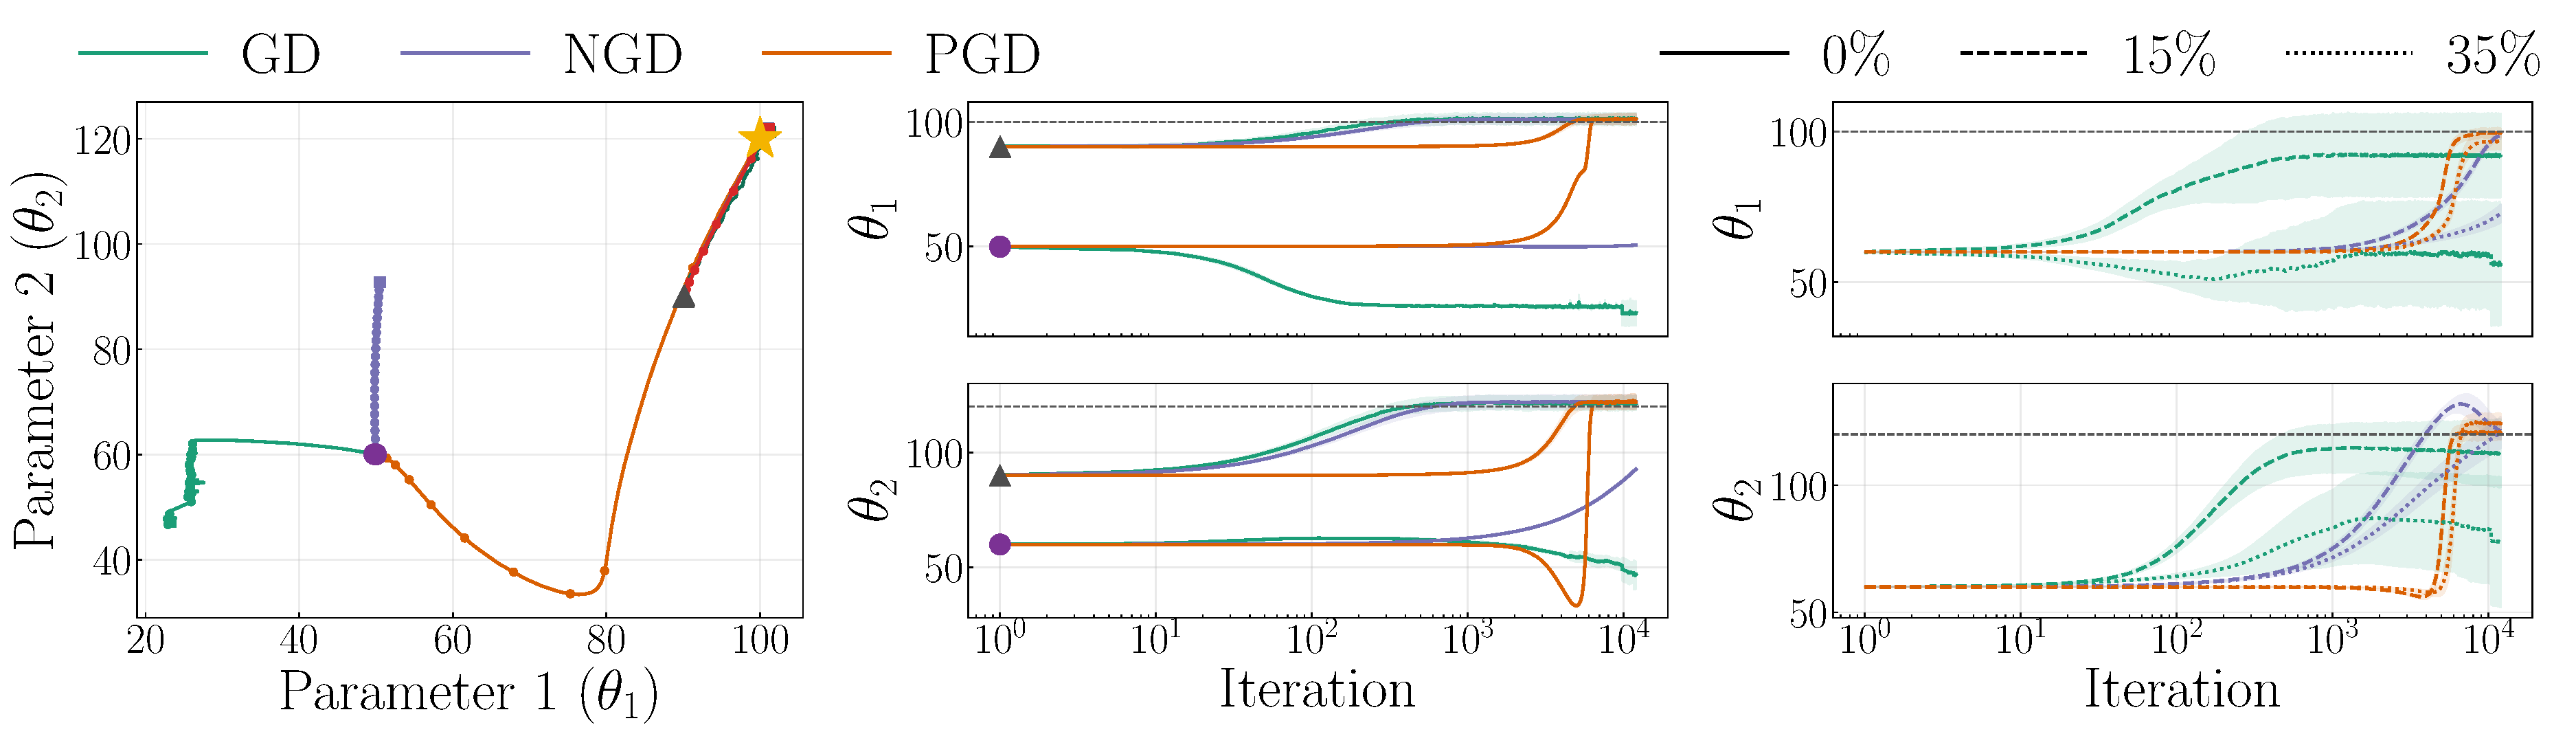
\includegraphics[width=0.99\linewidth]{figures/mdf_al_lotka_volterra_summary.pdf}
    \vspace{0.08cm}
    \begin{itemize}
        \small
        \item We compare gradient descent (GD), natural gradient descent (NGD)~\citep{briol2019statistical}, and preconditioned gradient descent (PGD, ours).
        \item First row: Close initialization. Second row: Far initialization.
    \end{itemize}
\end{frame}


\begin{frame}{Experiment: composite goodness-of-fit testing~\citep{key2025composite}}
    \begin{table}
        \centering
        \renewcommand{\arraystretch}{1.15}
        \begin{tabular}{lcc|cc}
            \toprule
            Method & Type-I error ($\downarrow$) & Time & Power ($\uparrow$) & Time \\
            \midrule
            PGD ($\mathcal{I}=1$) & 0.050 $\pm$ 0.018 & 8.6s & 0.829 $\pm$ 0.032 & 3.6s \\
            \midrule
            GD ($\mathcal{I}=400$) & 0.107 $\pm$ 0.026 & 10.4s & 0.600 $\pm$ 0.041 & 4.9s \\
            GD ($\mathcal{I}=1$) & 0.071 $\pm$ 0.022 & 2.6s & 0.279 $\pm$ 0.038 & 1.1s \\
            \bottomrule
        \end{tabular}
        \caption{\textit{Composite goodness-of-fit test.} $\mathcal{I}$ represents the number of restarts. }
    \end{table}
    \vspace{-0.15cm}
\end{frame}


\begin{frame}{Application: Generative models (WIP)}
    \centering
    \begin{minipage}[t]{0.185\linewidth}
        \centering
        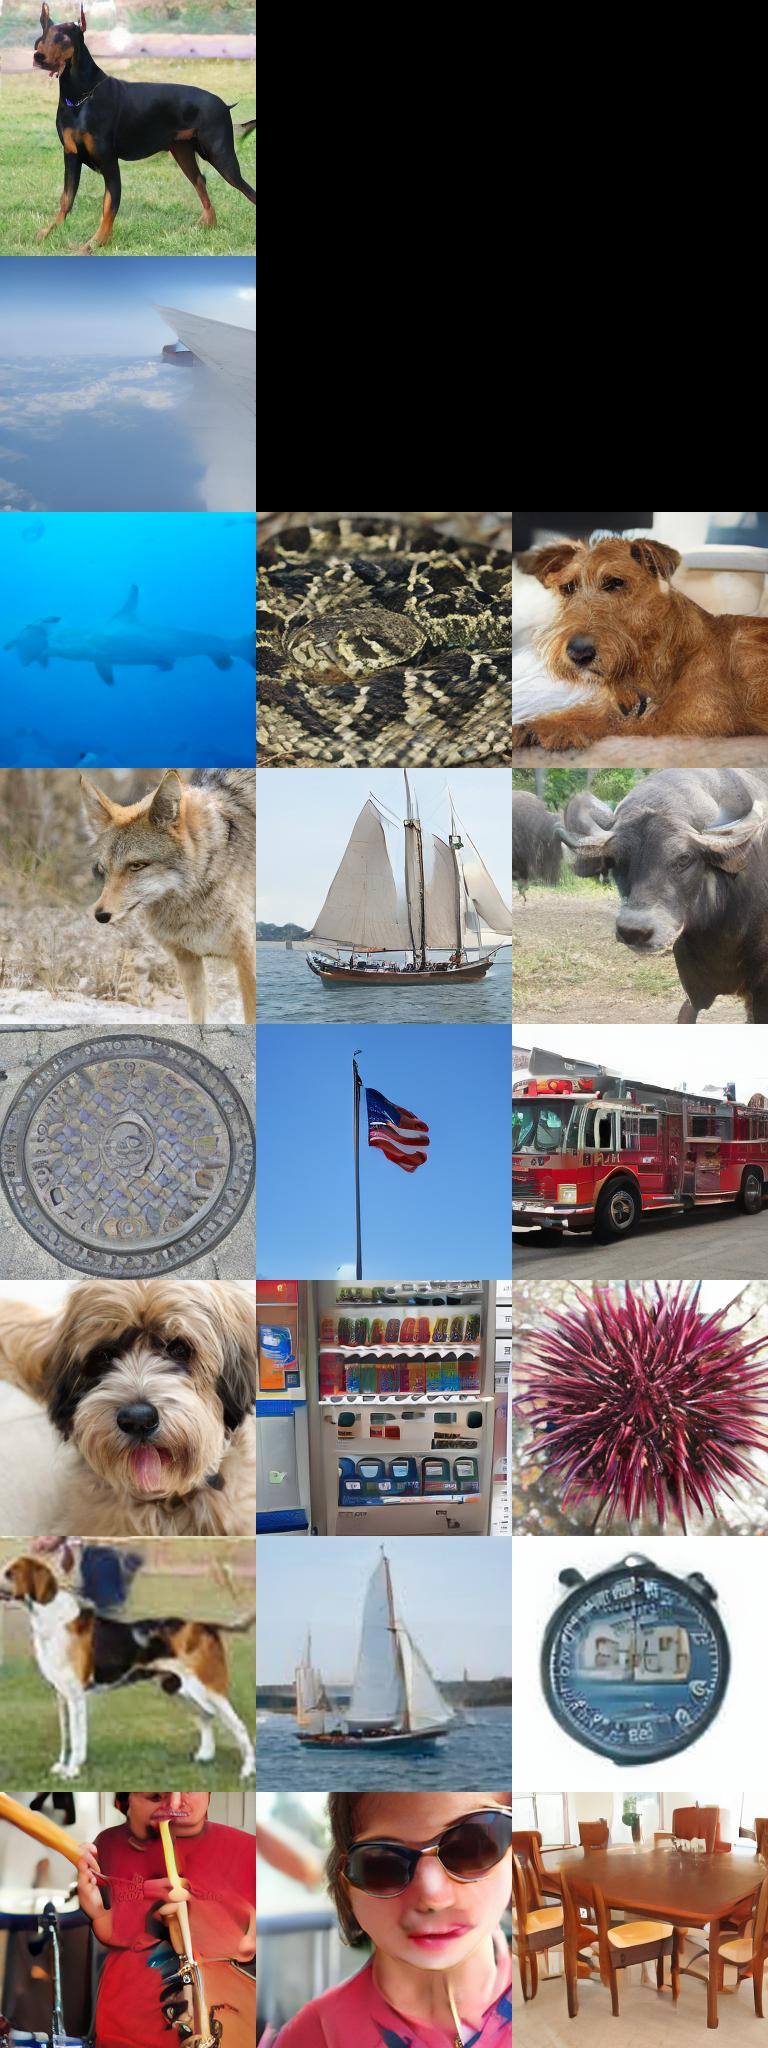
\includegraphics[width=\linewidth,trim={0 1536 512 256},clip]{figures/imagenet256_riesz_cfg2p5_step19999.jpg}\\[-0.02cm]
        {\scriptsize wing}
    \end{minipage}\hfill
    \begin{minipage}[t]{0.185\linewidth}
        \centering
        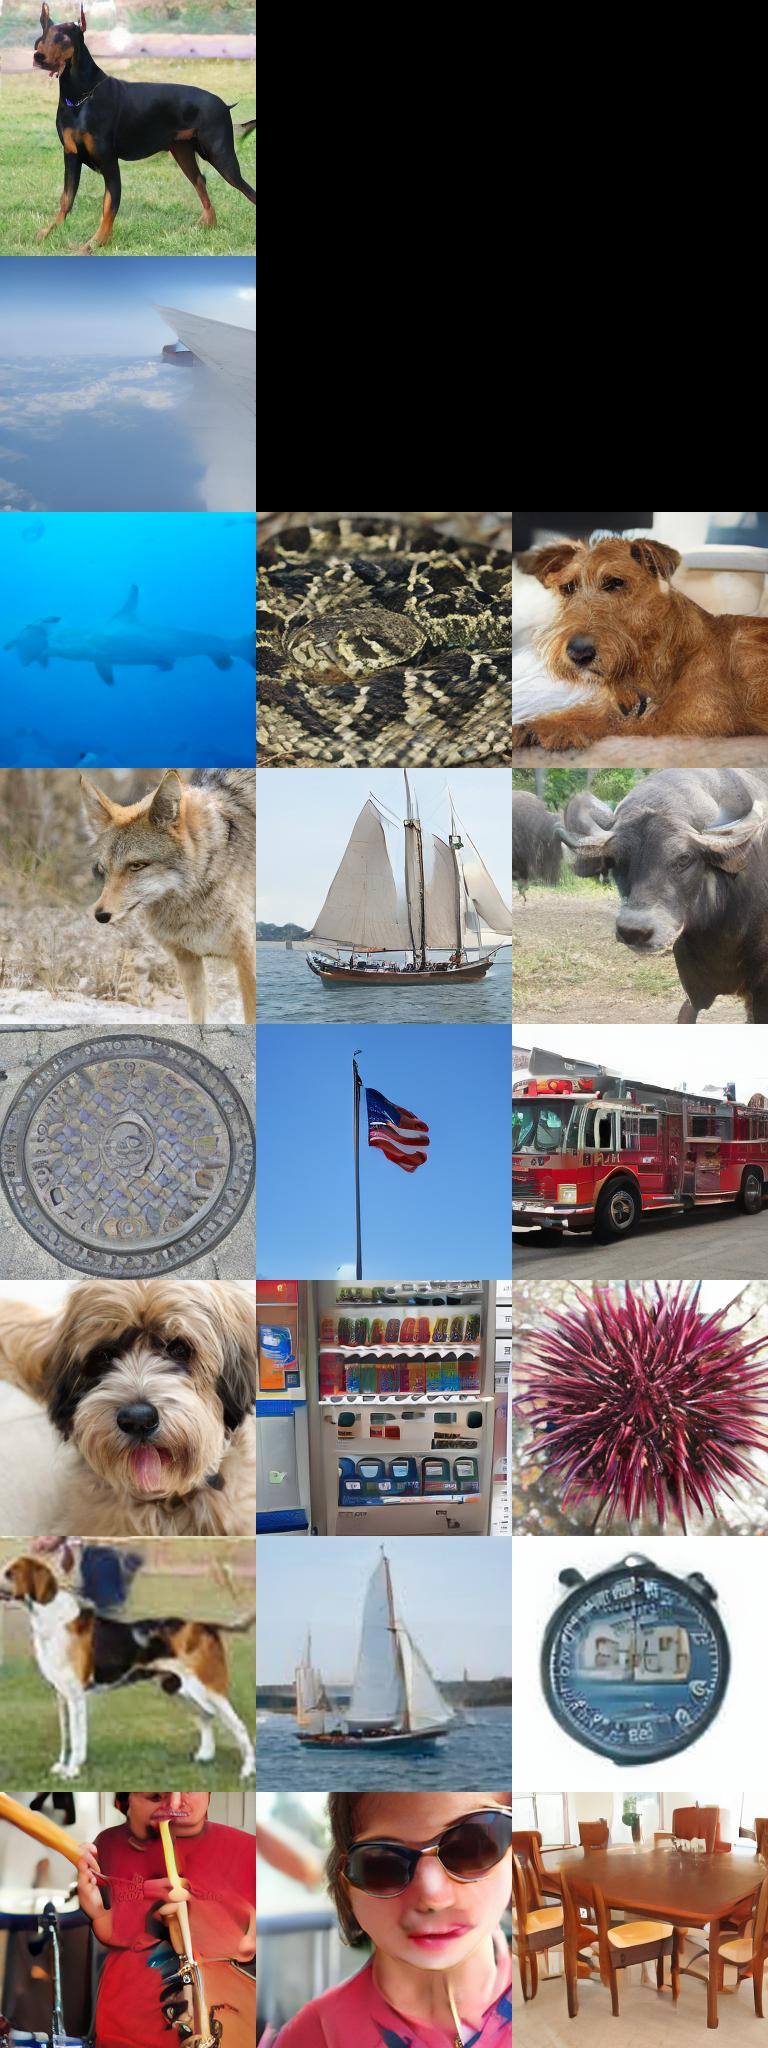
\includegraphics[width=\linewidth,trim={0 1280 512 512},clip]{figures/imagenet256_riesz_cfg2p5_step19999.jpg}\\[-0.02cm]
        {\scriptsize hammerhead shark}
    \end{minipage}\hfill
    \begin{minipage}[t]{0.185\linewidth}
        \centering
        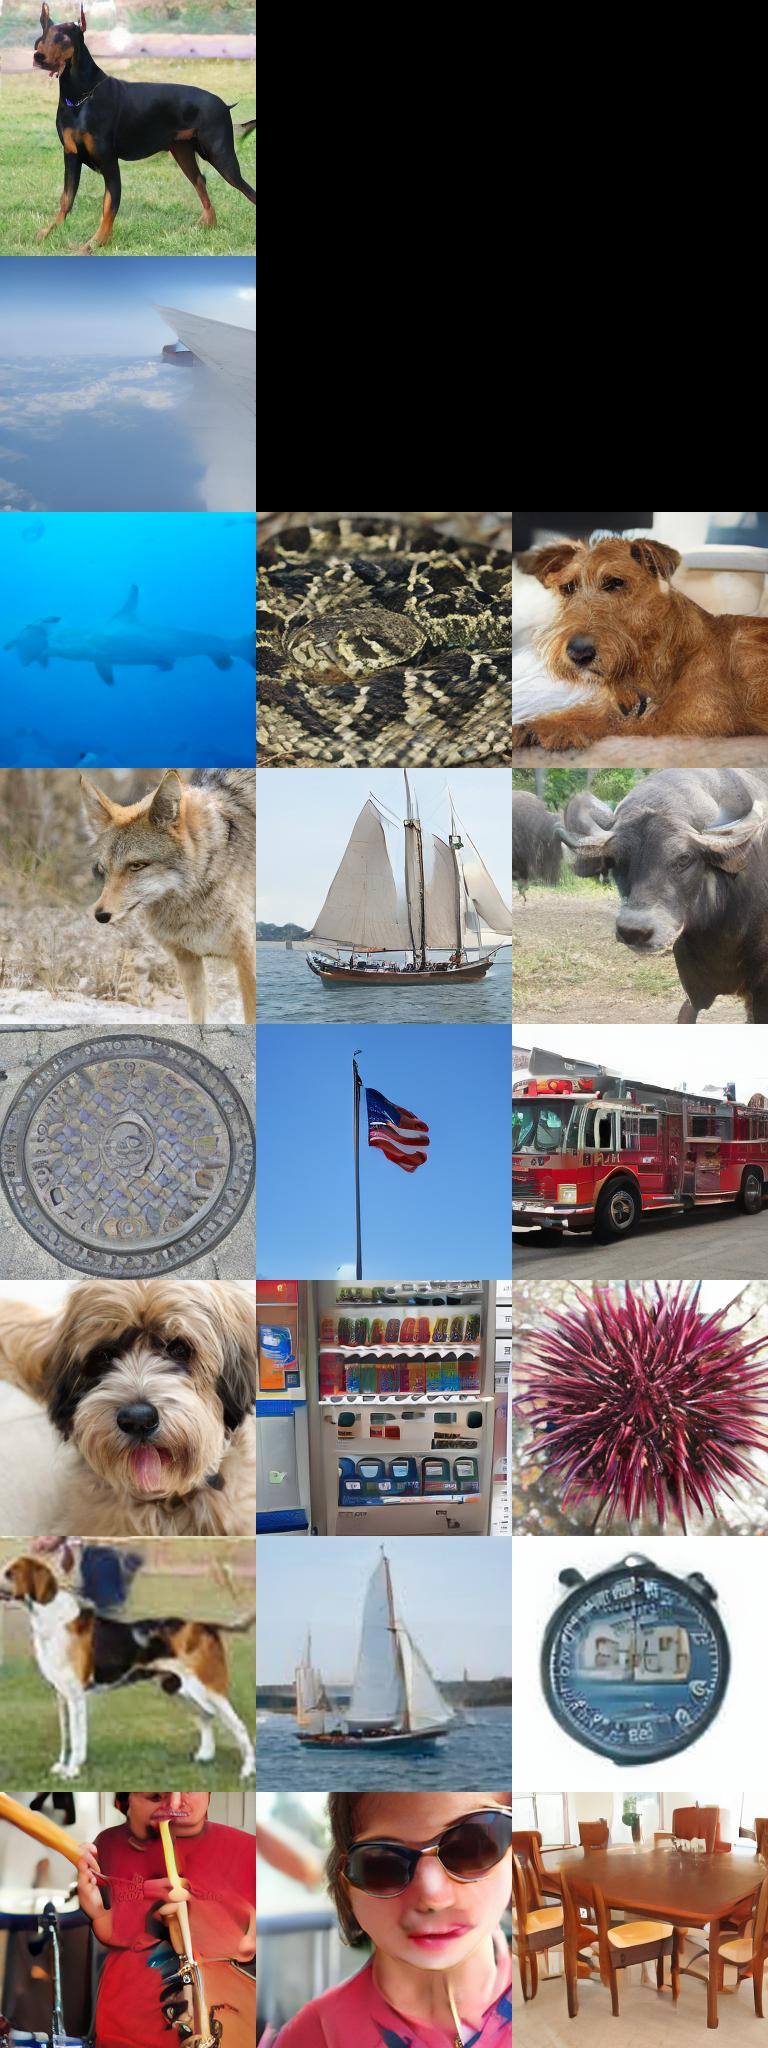
\includegraphics[width=\linewidth,trim={512 1280 0 512},clip]{figures/imagenet256_riesz_cfg2p5_step19999.jpg}\\[-0.02cm]
        {\scriptsize Irish terrier}
    \end{minipage}\hfill
    \begin{minipage}[t]{0.185\linewidth}
        \centering
        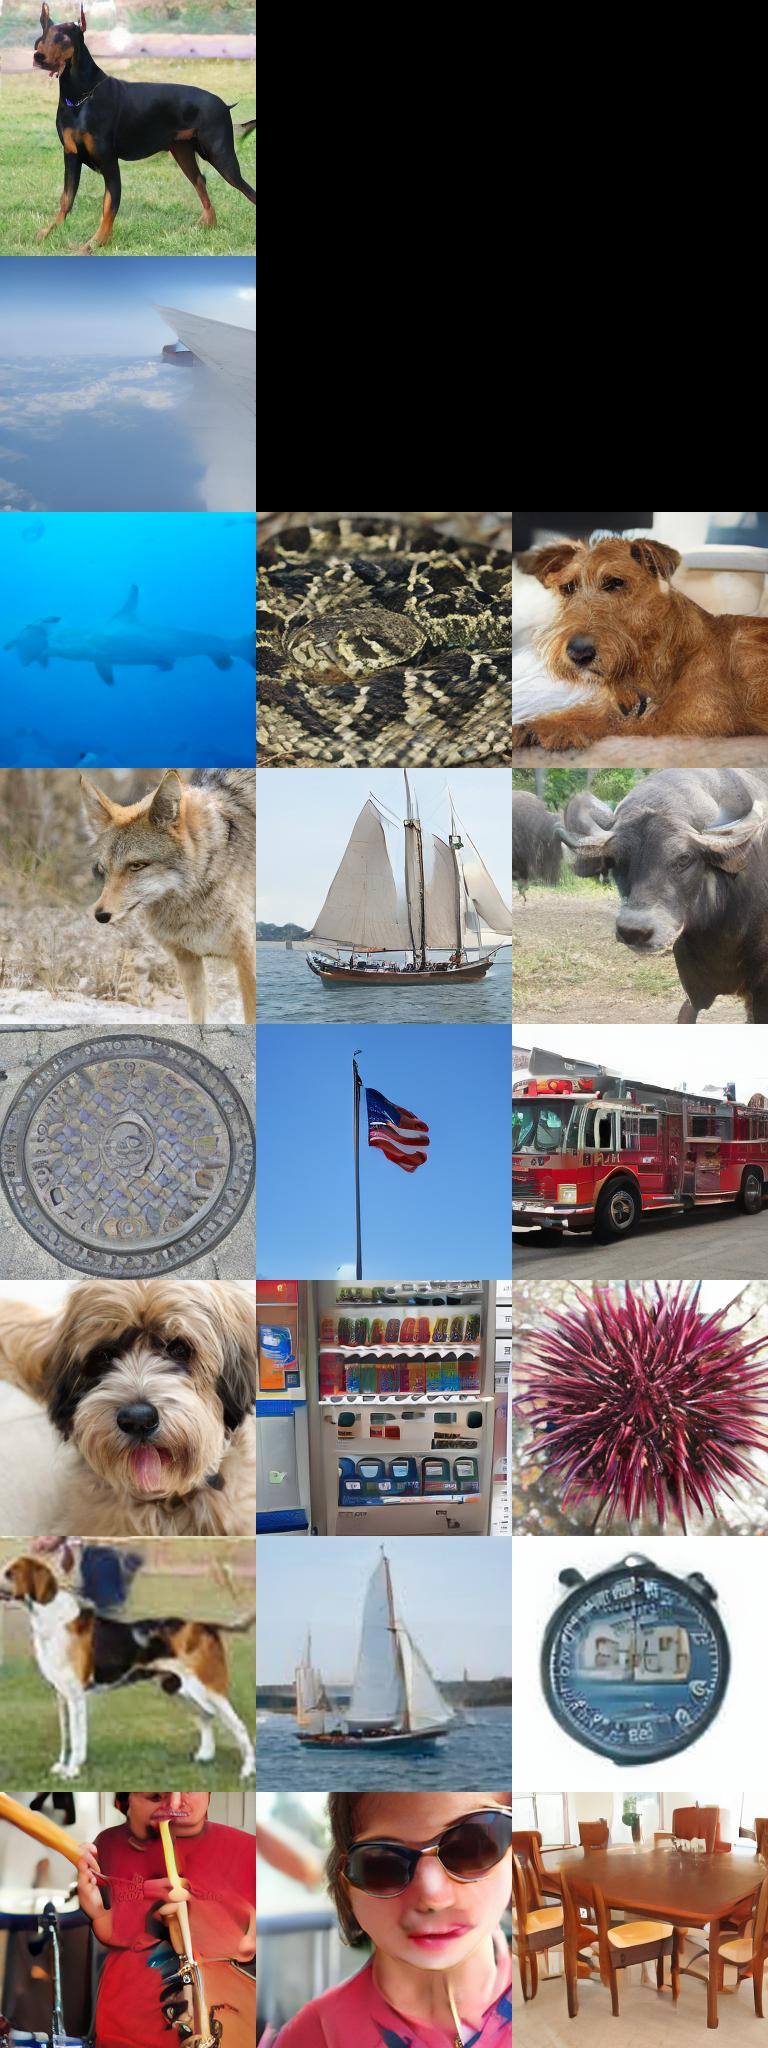
\includegraphics[width=\linewidth,trim={0 1024 512 768},clip]{figures/imagenet256_riesz_cfg2p5_step19999.jpg}\\[-0.02cm]
        {\scriptsize coyote}
    \end{minipage}\hfill
    \begin{minipage}[t]{0.185\linewidth}
        \centering
        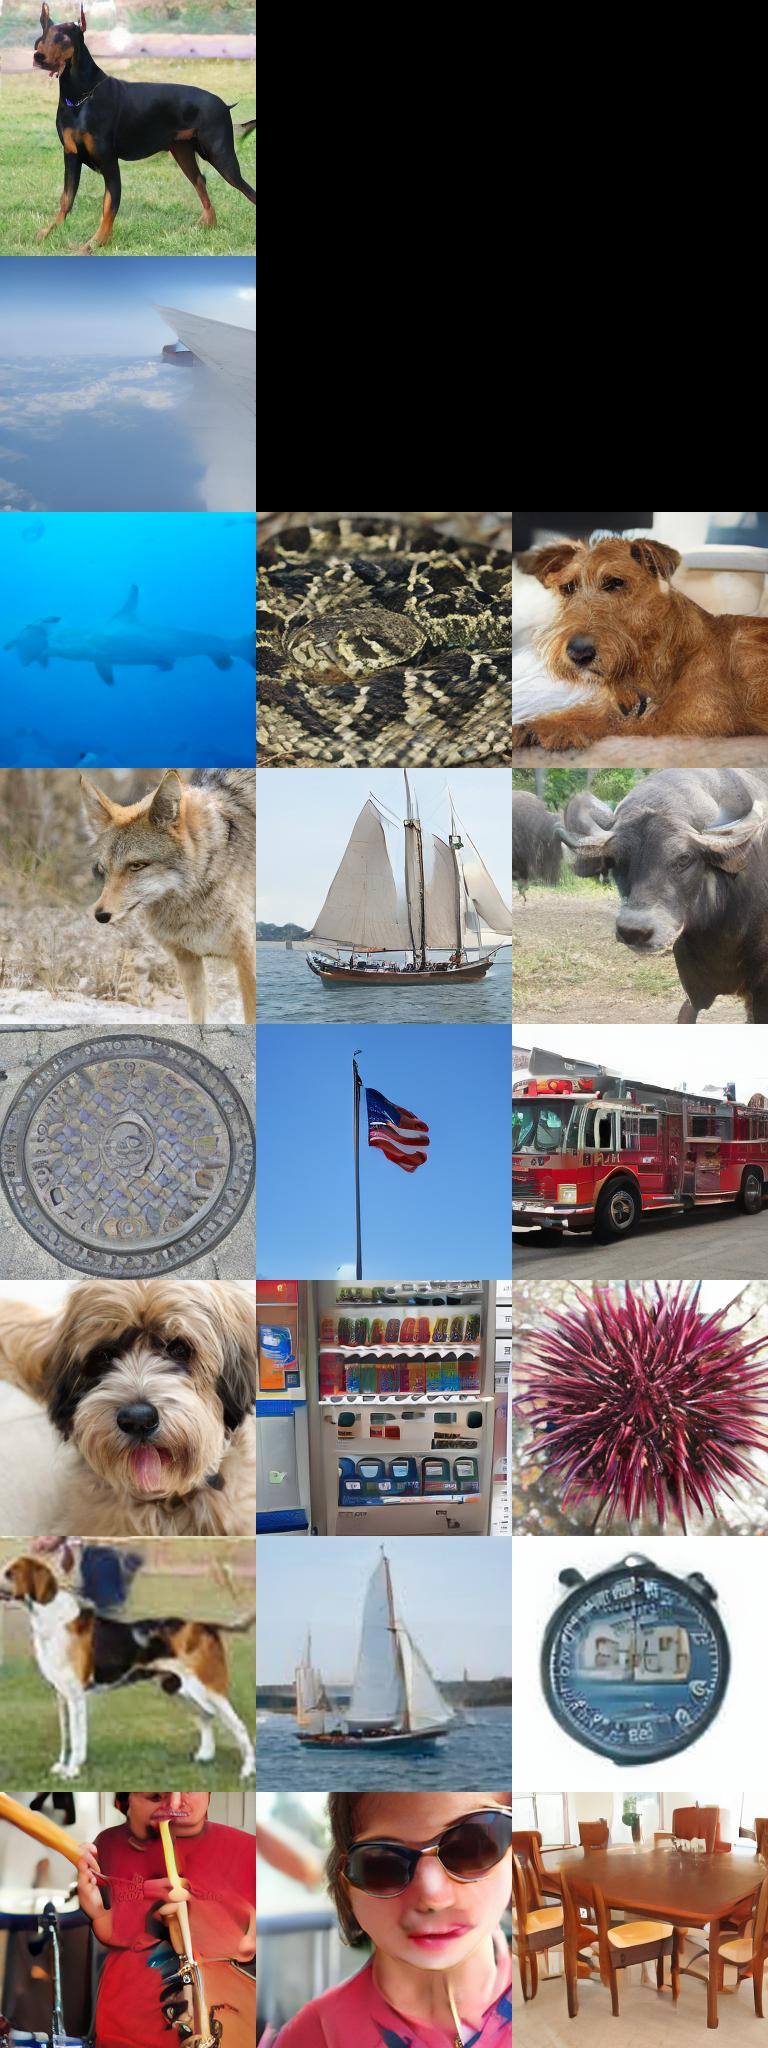
\includegraphics[width=\linewidth,trim={256 1024 256 768},clip]{figures/imagenet256_riesz_cfg2p5_step19999.jpg}\\[-0.02cm]
        {\scriptsize schooner}
    \end{minipage}

    \vspace{0.14cm}

    \begin{minipage}[t]{0.185\linewidth}
        \centering
        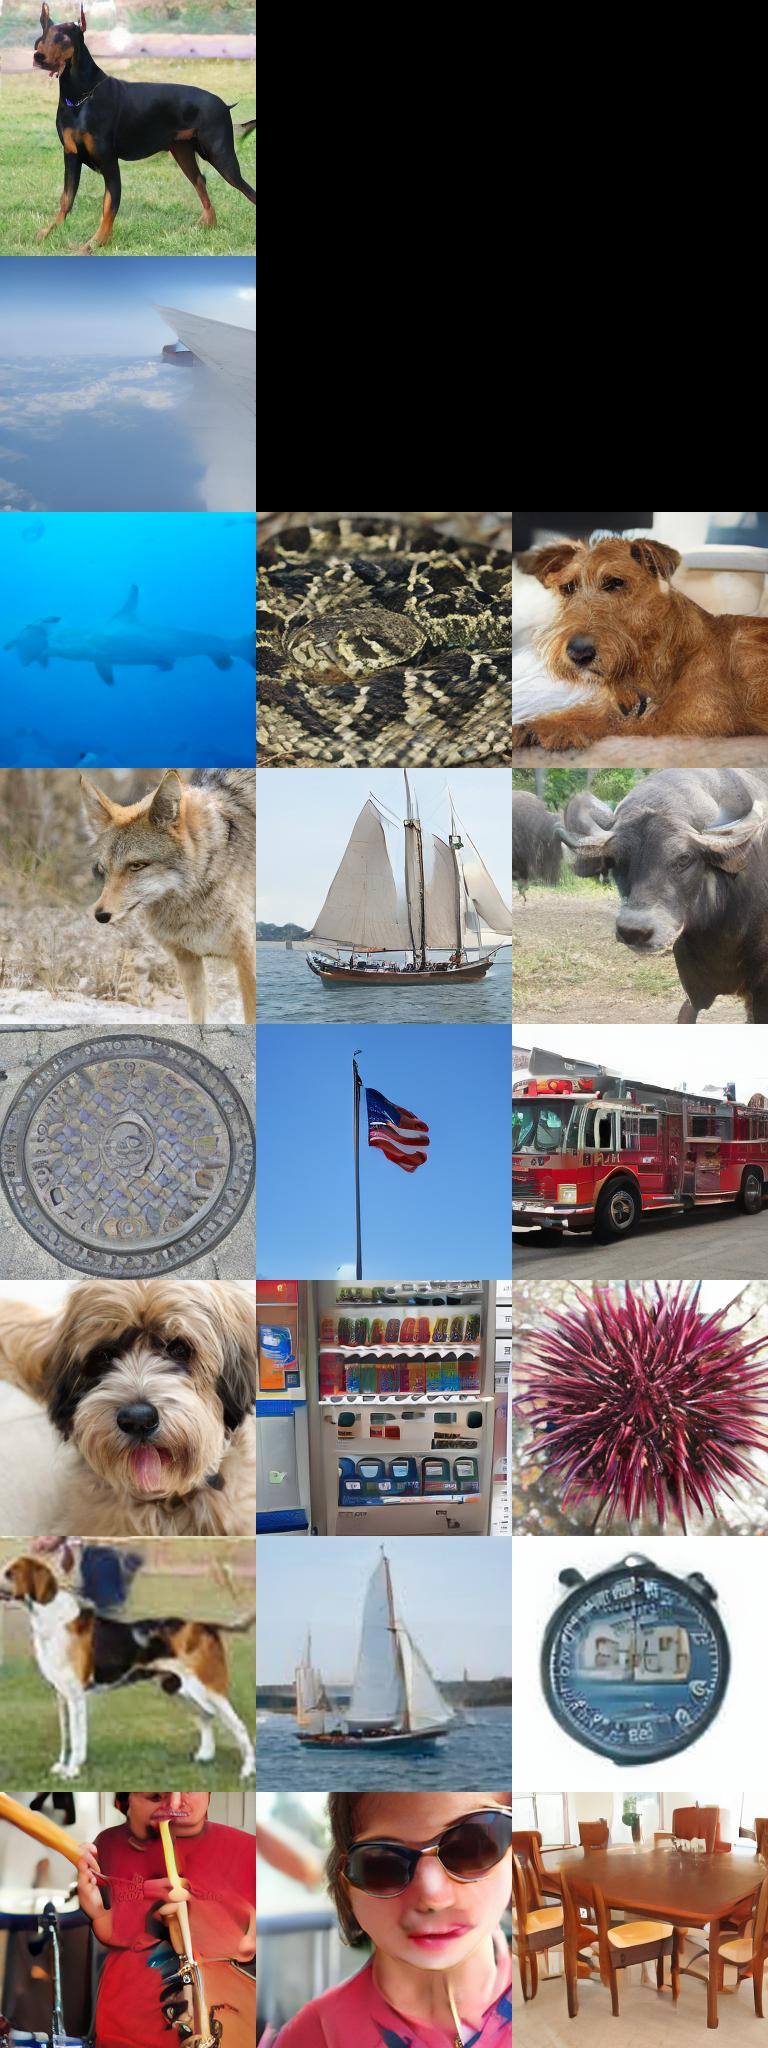
\includegraphics[width=\linewidth,trim={512 1024 0 768},clip]{figures/imagenet256_riesz_cfg2p5_step19999.jpg}\\[-0.02cm]
        {\scriptsize water buffalo}
    \end{minipage}\hfill
    \begin{minipage}[t]{0.185\linewidth}
        \centering
        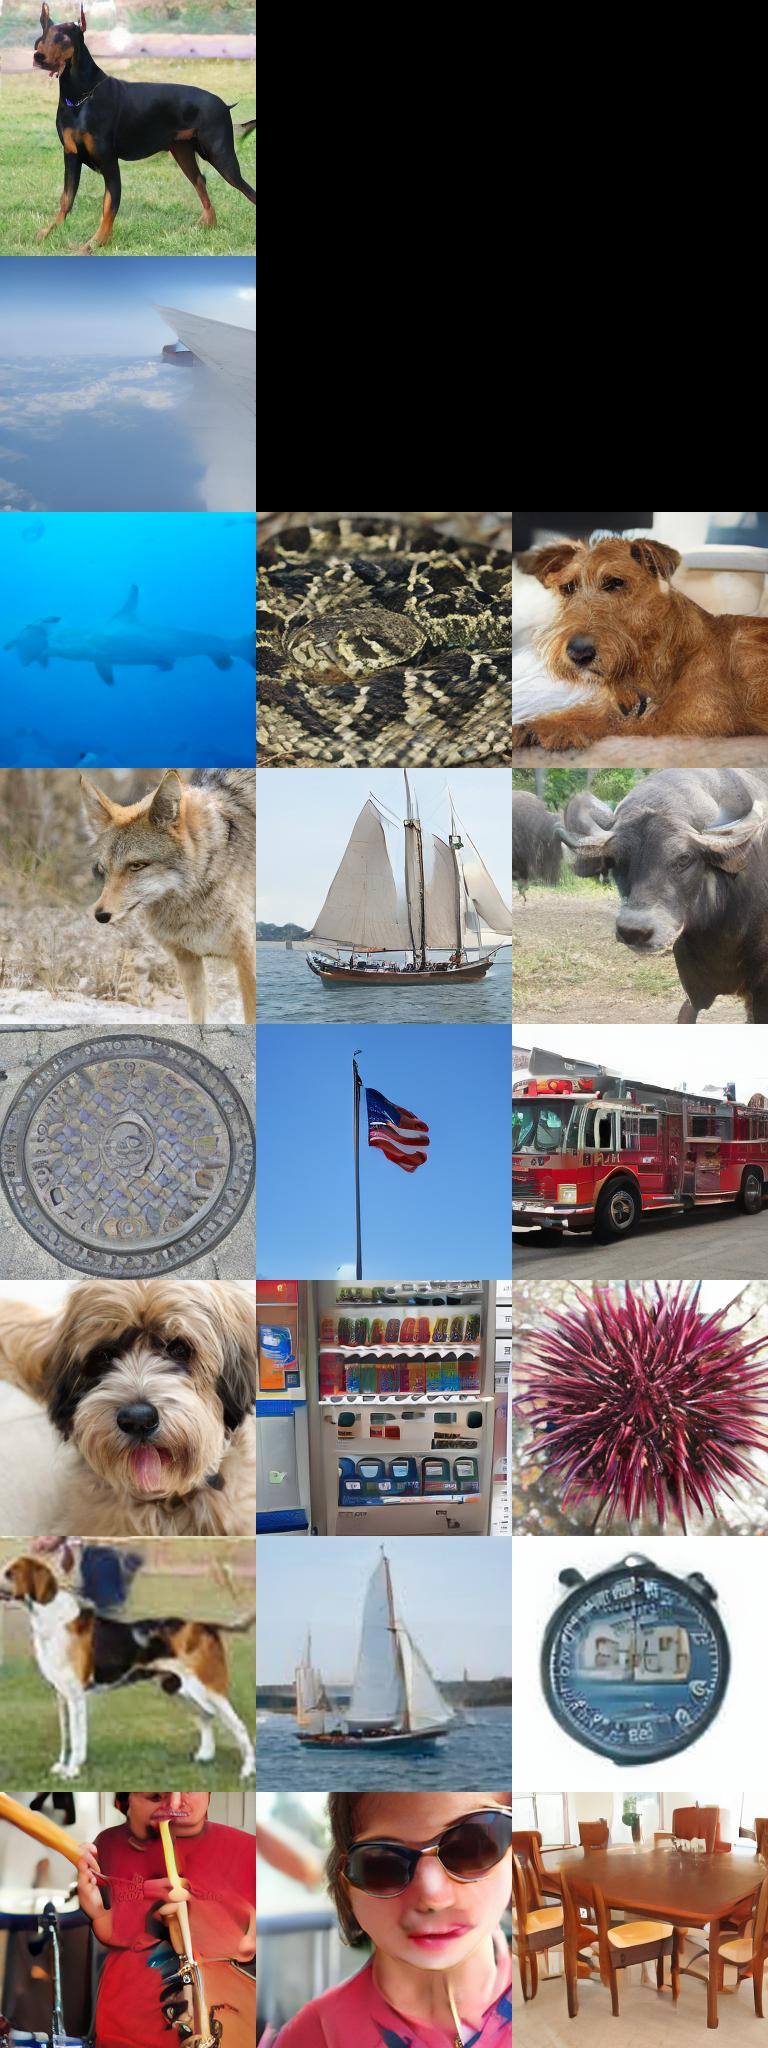
\includegraphics[width=\linewidth,trim={0 768 512 1024},clip]{figures/imagenet256_riesz_cfg2p5_step19999.jpg}\\[-0.02cm]
        {\scriptsize manhole cover}
    \end{minipage}\hfill
    \begin{minipage}[t]{0.185\linewidth}
        \centering
        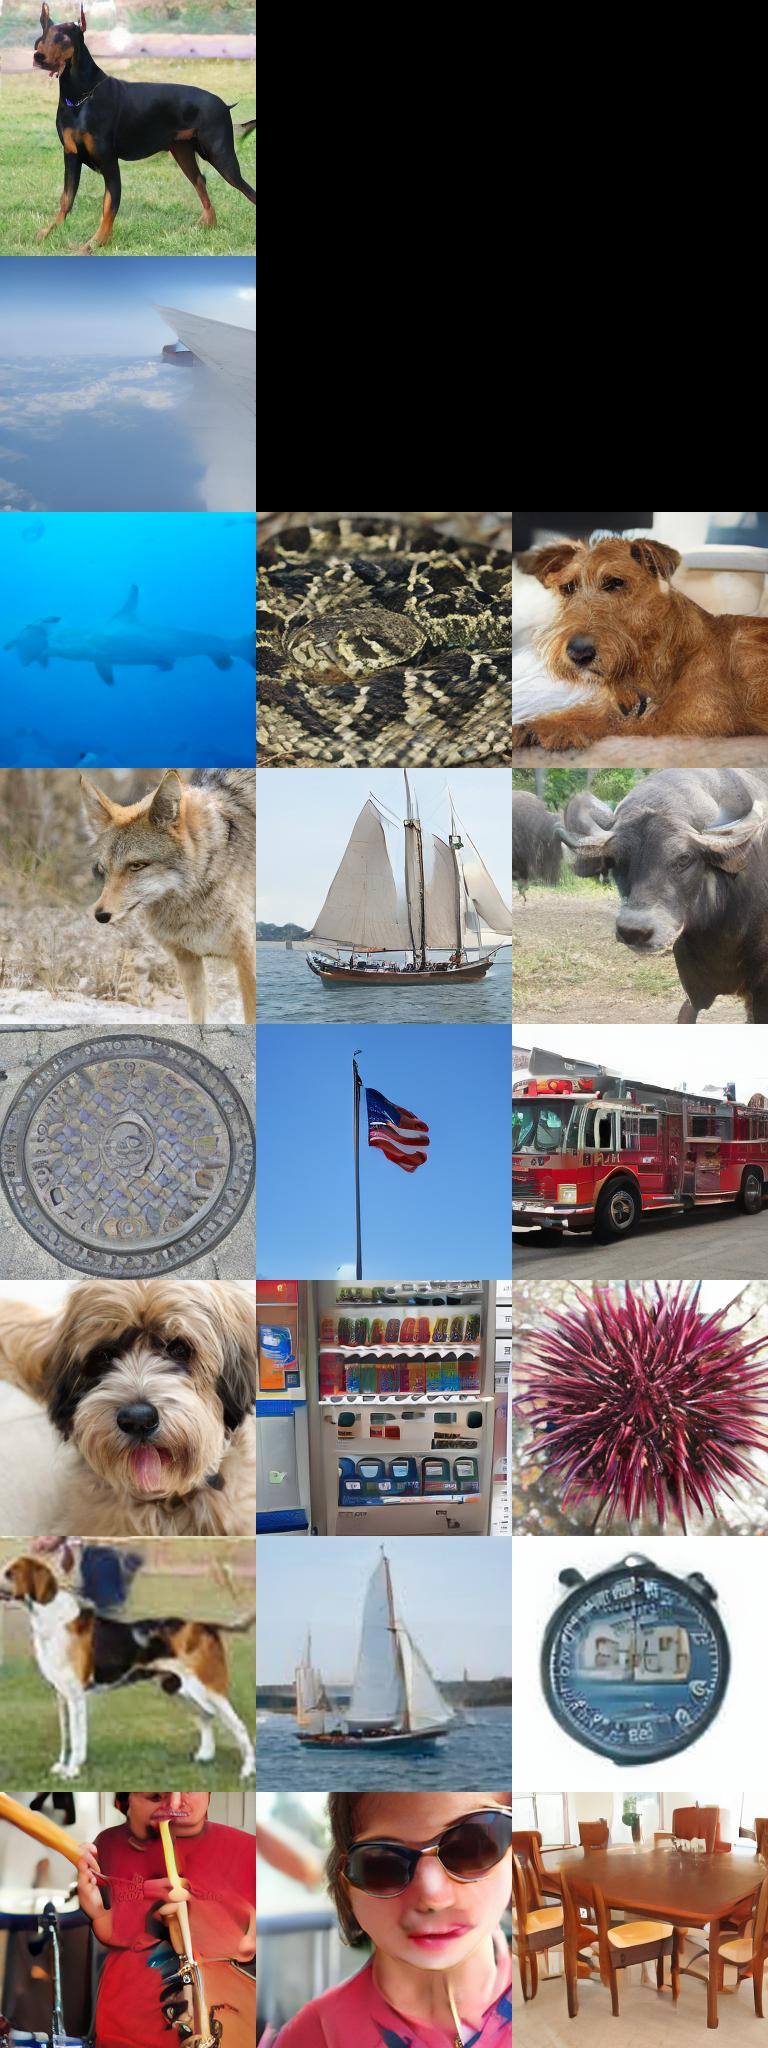
\includegraphics[width=\linewidth,trim={512 768 0 1024},clip]{figures/imagenet256_riesz_cfg2p5_step19999.jpg}\\[-0.02cm]
        {\scriptsize fire engine}
    \end{minipage}\hfill
    \begin{minipage}[t]{0.185\linewidth}
        \centering
        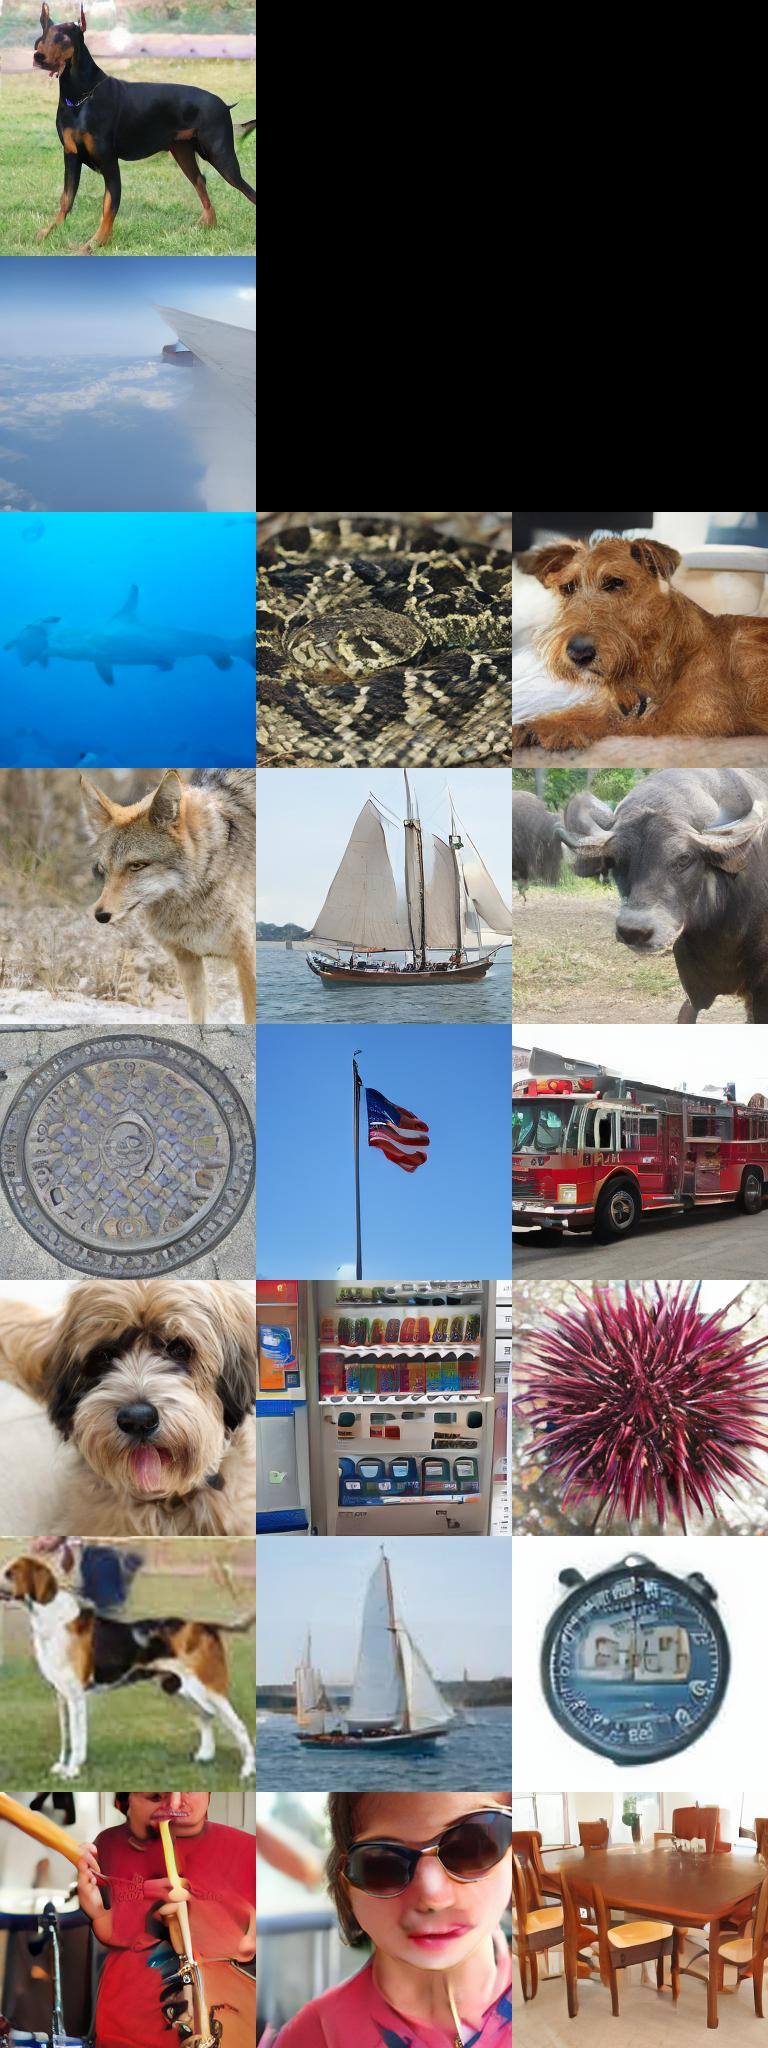
\includegraphics[width=\linewidth,trim={256 512 256 1280},clip]{figures/imagenet256_riesz_cfg2p5_step19999.jpg}\\[-0.02cm]
        {\scriptsize vending machine}
    \end{minipage}\hfill
    \begin{minipage}[t]{0.185\linewidth}
        \centering
        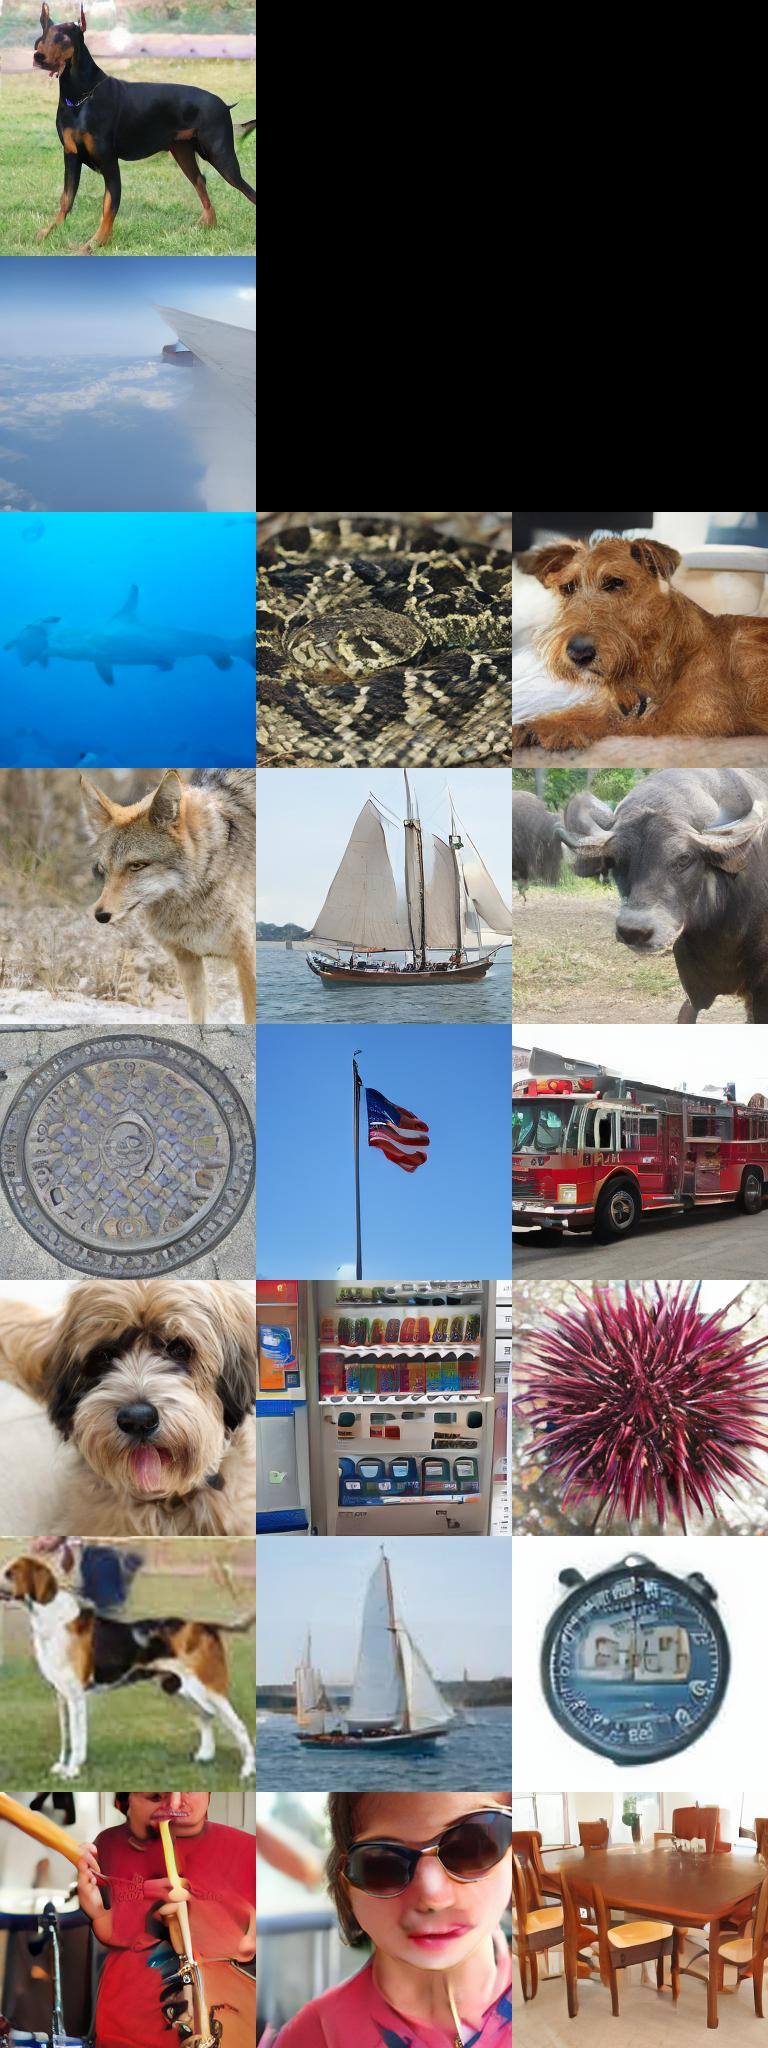
\includegraphics[width=\linewidth,trim={512 0 0 1792},clip]{figures/imagenet256_riesz_cfg2p5_step19999.jpg}\\[-0.02cm]
        {\scriptsize dining table}
    \end{minipage}

    \vspace{0.12cm}

    \begin{itemize}
        \item ResNet-style encoder pre-trained with masked autoencoding (MAE)~\citep{deng2026generative}.
    \end{itemize}
\end{frame}

\section{Conclusions}
\begin{frame}{Conclusions}
\begin{itemize}
    \item Minimization of MMD
    \begin{itemize}
        \item Interpolation towards $\chi^2$: $$\operatorname{DrMMD}(\Pb, \Qb)=\sup _{f \in \mathcal{H}:\|f\|_{L_2(\Pb)}^2+\lambda\|f\|_{\mathcal{H}}^2 \leq 1} \int f \mathrm{~d}(\Pb-\Qb)$$.
        \item Gradient penalty: $$\operatorname{SrMMD}(\Pb, \Qb)=\sup _{f \in \mathcal{H}:\|\nabla f\|_{L_2^d(\Pb)}^2+\lambda\|f\|_{\mathcal{H}}^2 \leq 1} \int f \mathrm{~d}(\Pb-\Qb)$$.
    \end{itemize}
    \item Application I: Minimum MMD inference.
    \item Application II: One-step generative models.
\end{itemize}
\end{frame}


\section{Personal}
\begin{frame}{About Me}
  \begin{columns}[c] % 'c' aligns vertically center
    % Left column with image
    \column{0.4\textwidth}
    \centering
    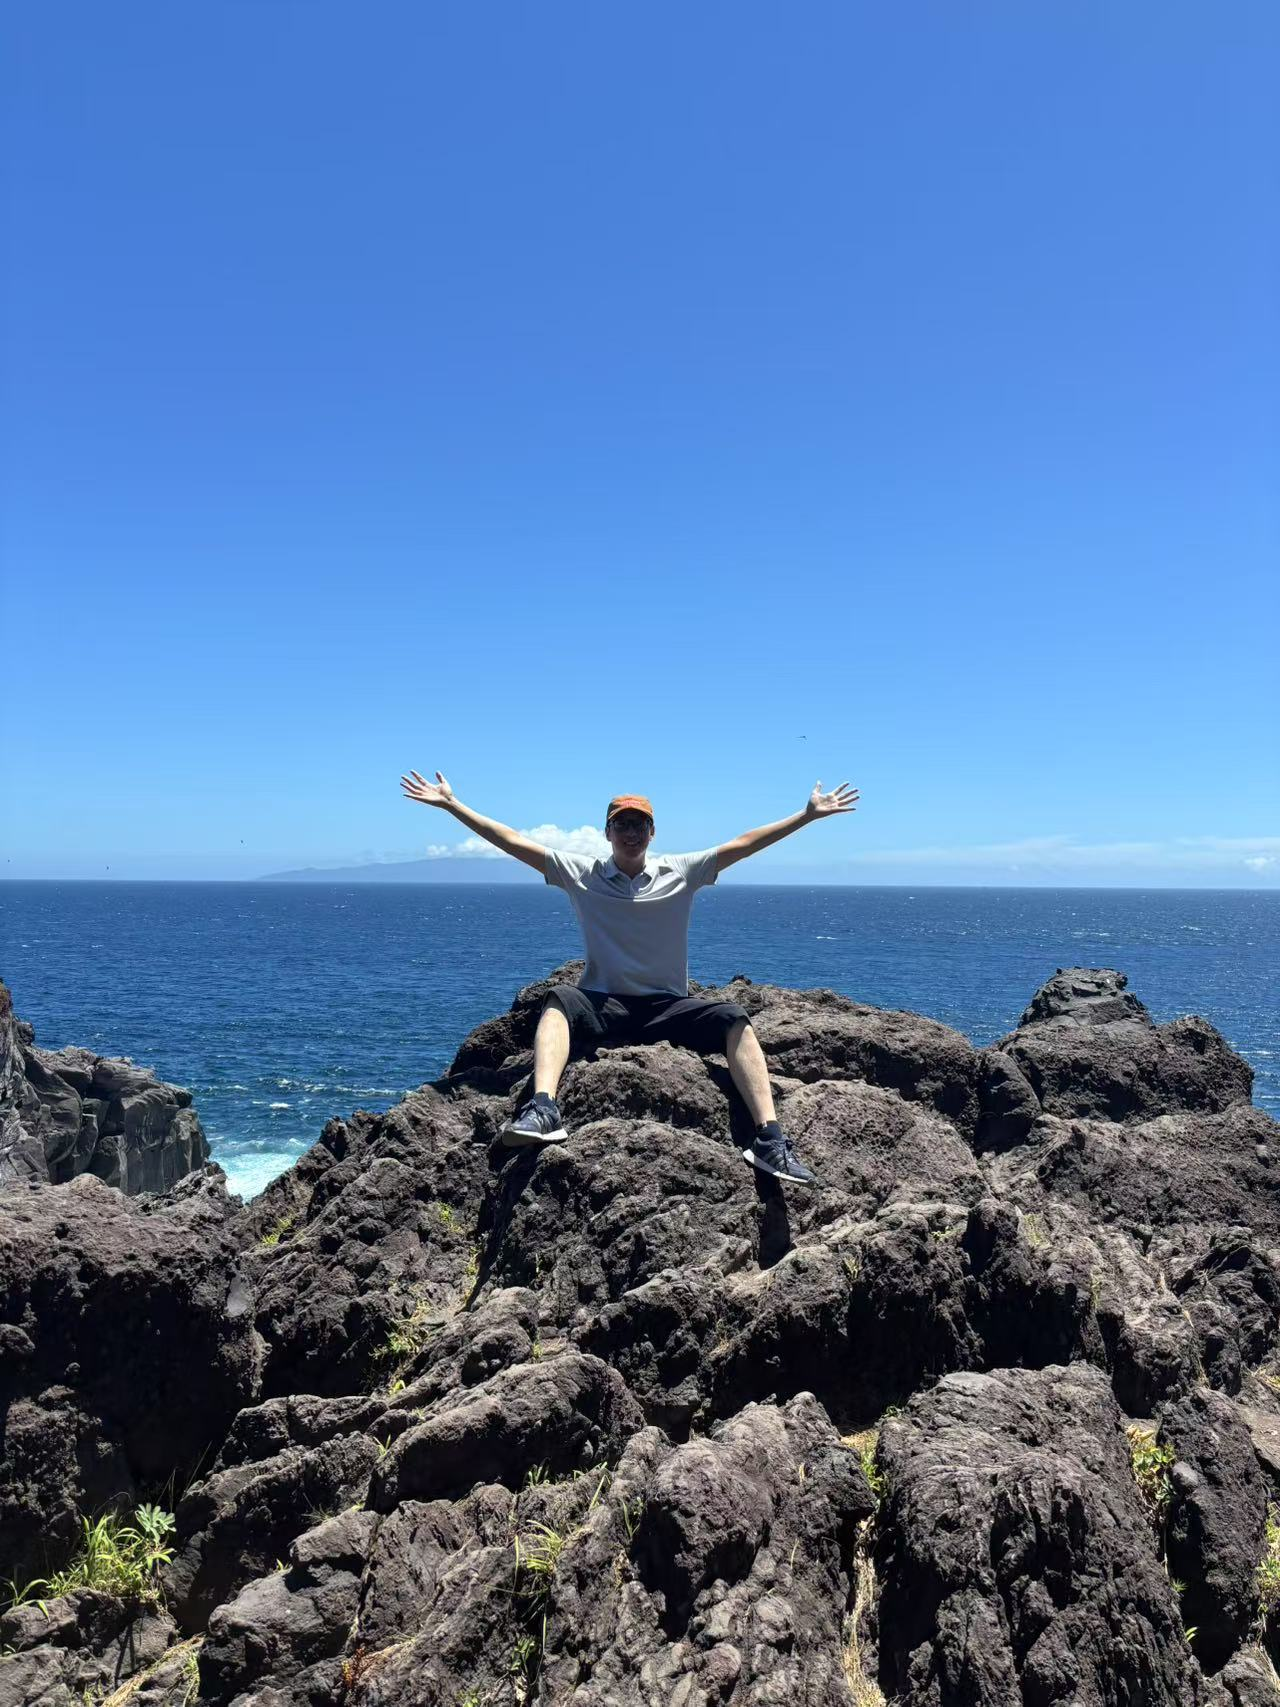
\includegraphics[width=0.9\linewidth]{figures/personal.png}
    \column{0.6\textwidth}
    \begin{itemize}
        \item Zonghao Chen
        \item 4th year PhD Student at University College London (UCL)
        \begin{itemize}
            \item Foundational AI Centre
            \item Gatsby Computational Neuroscience Unit
        \end{itemize}
        \item Graduated from Tsinghua University in 2022
        \begin{itemize}
            \item Department of EE
        \end{itemize}
        \item Kernel (nonparametric) methods, causal inference, statistical learning theory
    \end{itemize}
  \end{columns}
\end{frame}


\bibliographystyle{alpha}
\bibliography{reference}

\end{document}
